%Programma previsto
% Dinamica: dinamica del punto materiale (3 leggi dinamica)
% Meccanica: quantita' conservative (energia ecc)
% Termodinamica dei gas
% Entropia/probabilita'/senso del tempo
% Elettricita': Coulomb
% Magnetismo



% storico LEZIONI

% PARTE: INTRODUZIONE ALLA FISICA

% Lezione 01/2024-02-26
% - Introduzione filosofica alla fisica (di che si occupa, rapporto con la realta' e filosofia della quantificazione, metodo scientifico)
% - Quantificazione: misura ed errore di misura, stima

% PARTE: CINEMATICA DEL PUNTO

% Lezione 02/2024-02-28
% - Notazioni sulla quantificazione: ordine di grandezza
% (include altri argomenti, ma con un capitolo dedicato)
% - Introduzione alla descrizione quantitativa del moto (cinematica?)
% - cinematica del punto materiale da una a piu' dimensioni: moto rettilineo uniforme, piano cartesiano
% - equazioni del moto, con notazione vettoriale
% Esercitarsi su: moto rettilineo uniforme, vettori e trigonometria, sistemi di riferimento cartesiani e algebra sul piano cartesiano

% PARTE: DINAMICA

% Lezione 03/2024-03-04
% - introduzione alla dinamica
% - prima e seconda legge
% - esercizi su moto uniformemente accelerato
% - accenni al concetto di forza e introduzione alla forza elastica con legge di hooke

% Lezione 04/2024-03-06
% - grafico orario: grafico nel quale un asse riporta lo spazio (una dimensione), mentre sull'altro il tempo
% - differenza tra SPOSTAMENTO e distanza
% - interpretazione grafica della velocità e accelerazione, con analisi di funzione

% Lezione 05/2024-03-11
% - moto del punto nel piano
% - sistema di riferimento con vettore posizione
% - accelerazione in moti con traiettoria curvilinea
% - la STATICA si occupa della quiete

% Lezione 06/2024-03-13
% - introduzione al moto armonico
% - pendolo

% Lezione 07/2024-03-18
% - moto armonico (equazioni, con condizione sufficiente per un moto armonico)
% - oscillatore armonico a molla

% PARTE: MECCANICA

% Lezione 08/2024-03-20
% - lavoro di una forza
% - teorema delle forze vive, con dimostrazione
% - energia cinetica

% Lezione 09/2024-03-25
% - introduzione energia pontenziale (gravitazionale e elastica)
% - introduzione a forze conservative e nonZZZzzzZZZzzzZZZzzz

% Lezione 10/2024-03-27
% - CONSERVAZIONE DELL'ENERGIA MECCANICA
% - significato dell'energia potenziale
% - teorema della conservazione dell'energia meccanica

% Lezione 11/2024-04-01 Pasquetta






% Lezione 12-11/2024-04-03
% - URTI E QUANTITA DI MOTO
% - legge di conservazione della qtà di moto
% - reversibilità della meccanica
% - biliardo
% - centro di massa
% - impulso

% Lezione 13-12/2024-04-08
% - SISTEMI DI RIFERIMENTO, intro alla relatività galileiana (in funzione dello studio del centro di massa)
% - urti anelastici, dimostrazione non-conservazione energ. cinetica
% - analisi dell'urto anelastico dal punto di vista del centro di massa

% Lezione 14/2024-04-10 Saltata per qualche motivo
% Lezione 15/2024-04-15 Saltata per qualche motivo










% Lezione 16-13/2024-04-17
% - SISTEMI DI RIFERIMENTO E RELATIVITA' GALILEIANA
% - velocità di trascinamento
% - principio di relatività galileiana











%%%%% GRAVITAZIONE E TERMODINAMICA %%%%%%%%%

% Lezione 17-14/2024-04-22
% - ripasso sulla massa inerziale e seconda legge di newton
% - forze fondamentali conosciute oggi
% - TERMODINAMICA: intro e definizioni (sistema termotidamico, variabili termodinamiche, equilibrio termodinamico)

% Lezione 18/2024-04-24 % Saltata per qualche motivo

% Lezione 19-15/2024-04-29
% - temperatura e stati della materia (H2O, punto triplo)
% - definizione e calibrazione del termometro, scale termometriche K, °C, °F
% - principi 0 e I della termodinamica
% - contatto termico, pareti adiabatiche e diatermiche
% - esperienza di Joule e intuizione legame temperatura-lavoro-energia
% - printcipio I termodinamica, energ. interna - lavoro - calore
% - convenzione segni di lavoro e calore in un sistema termodinamico
% - capacità termica e calore specifico, esercizi con T di equilibrio, cambio di stato, calore latente
% - cenni sulla dilatazione termica (esercizio)

% Lezione 20/2024-05-01 Festa del lavoro

% Lezione 21-16/2024-05-06
% - dipendenza dell'energia interna unicamente dallo stato
% - approssimazione della curva di trasformazione: QUASISTATICA
% - trasformazione reversibile
% - fasi e stati di aggregazione della materia, cambiamento di fase (esempio dell'acqua)
% - calore latente
% - trasferimento del calore: conduzione, convezione, irraggiamento
% - vaso di dewar, legge di StefanBoltzman
% - gas: leggi notevoli di trasformazione
% - legge di avogadro, legge gas ideali/perfetti

% Lezione 22-17/2024-05-08
% - lavoro di un gas: lo stantuffo
% - joule e l'espansione libera dei gas
% - teoria cinetica dei gas: origine della pressione, energia interna del gas, energia cinetica
% - gradi di libertà

% Lezione 23-18/2024-05-13
% - trasformazioni termodinamiche
% - lavori, calore, calori specifici di gas ideali in trasformazioni
% - introduzione ai cicli termodinamici
% - relazione di Mayer

% Lezione 24-19/2024-05-15
% - macchine termiche, funzionamento tra sorgenti
% - ciclo di carnot, risultati di Carnot
% - ciclo Diesel e di 8
% - rendimento di una macchina, coefficiente di prestazione
% - flussi di calore nelle macchine: macchine frigorifere e motori

% Lezione 25-20/2024-05-20
% - formulazioni del secondo principio della termodinamica
% - teoremi: carnot e clausius

% Lezione 26-21/2024-05-22
% - ENTROPIA, teorema dell'entropia

% Lezione 27-22/2024-05-27 CONCLUSIONE UFFICIALE DEL CORSO
% - Esercizi grossi grossi finali sulla termodinamica.


% Potenziali lezioni(niente elettromagnetismo...)
% Lezione 28-23/2024-05-29
% Lezione 29-24/2024-06-03
% Lezione 30-25/2024-06-05

\documentclass{book}
\usepackage{feynmanslop}

\title{Fisica}
\author{Zeno Saletti}
\date{\today}


\begin{document}


\begin{titlepage}
    \newgeometry{left = 0cm, right = 0cm, top = 0cm, bottom = 0cm}
    \pagecolor{brown}\afterpage{\nopagecolor}
    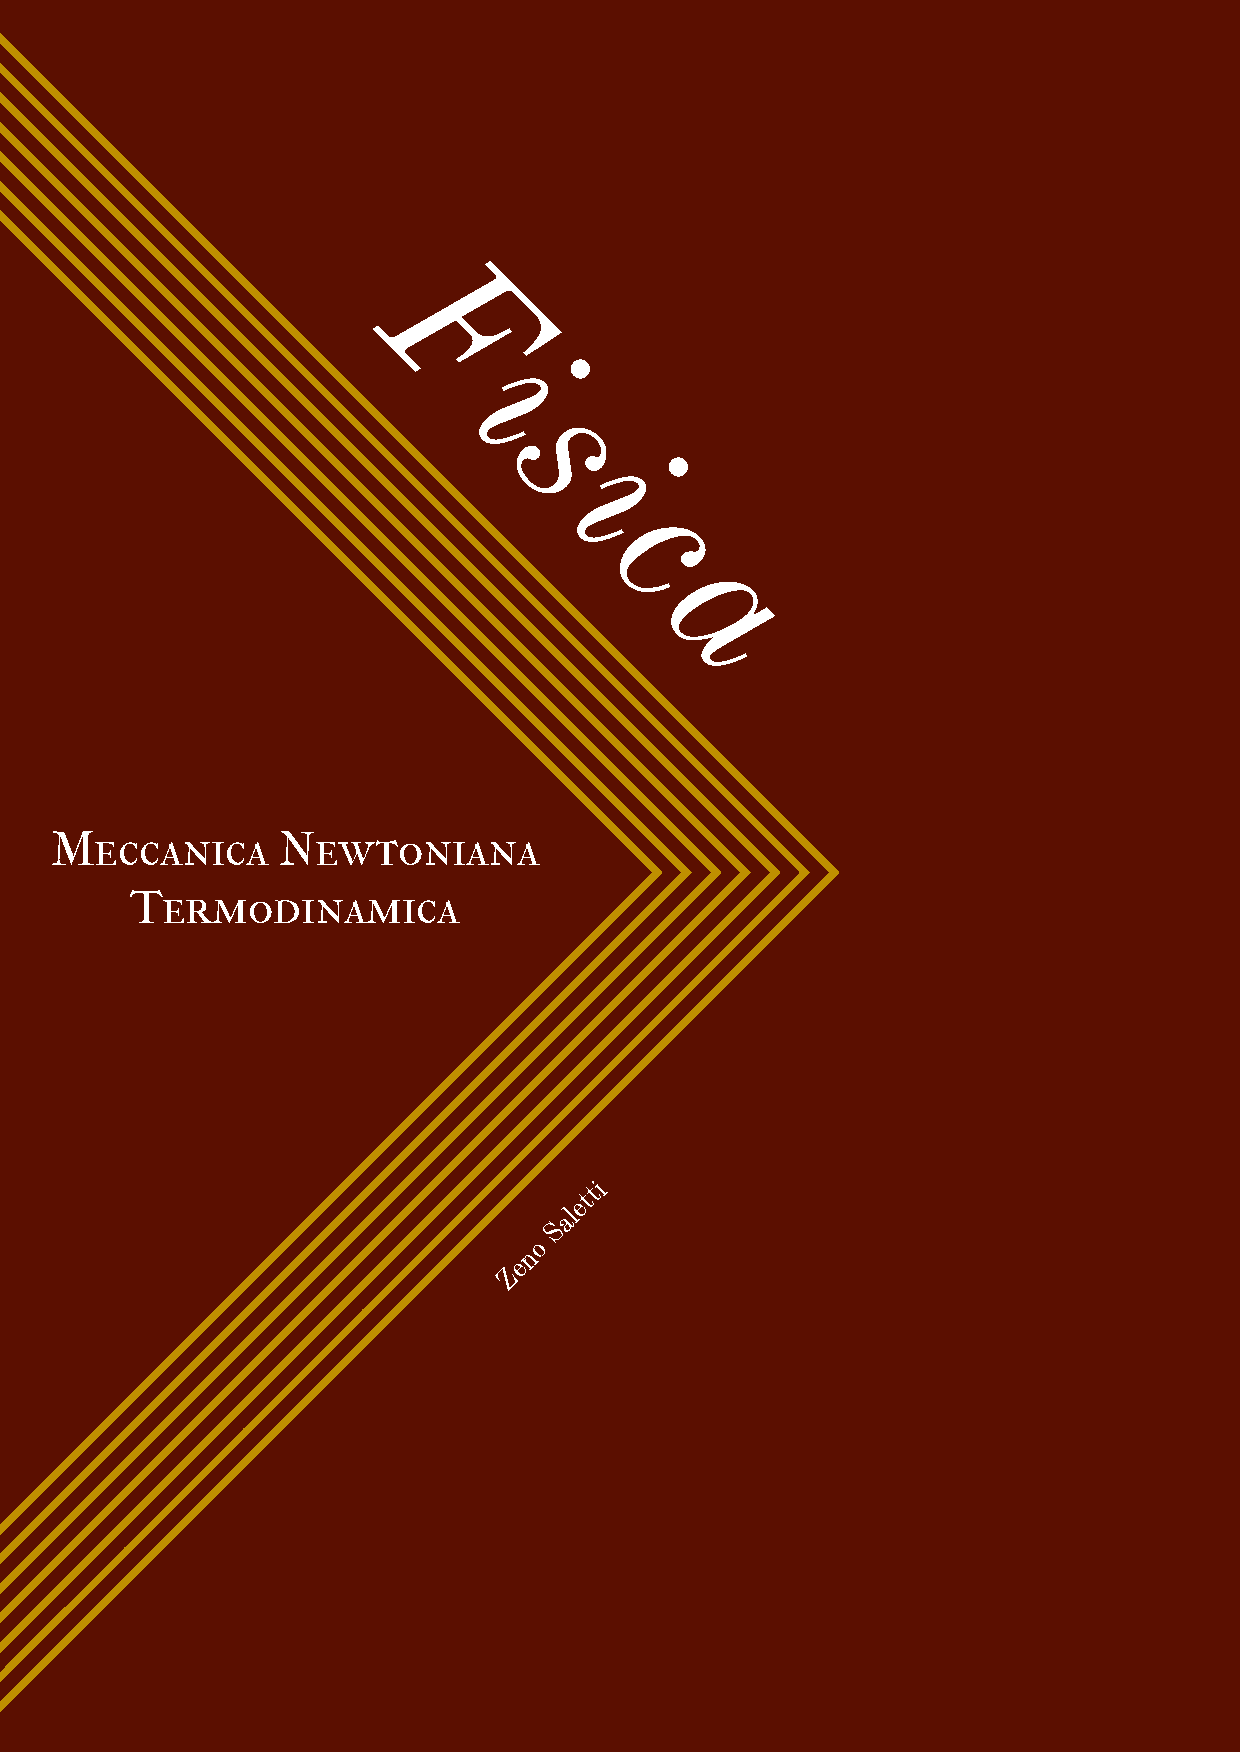
\includegraphics[width = \linewidth]{bookcover.pdf} % also works with logo.pdf

    \restoregeometry
\end{titlepage}

\epigraph{If, in some cataclysm, all of scientific knowledge were
to be destroyed, and only one sentence passed on to the next generations
of creatures, what statement would contain the most information in the
fewest words? I believe it is the \textit{atomic hypothesis} [...]
that \textit{all things are made of atoms—little particles that move
around in perpetual motion, attracting each other when they are a little
distance apart, but repelling upon being squeezed into one another.}
In that one sentence, you will see, there is an enormous amount of
information about the world, if just a little imagination and
thinking are applied.}{Richard P. Feynman,\\\textit{The Feynman Lectures on Physics}\\Vol. I}

\vspace*{9cm}
\begin{center}
Consigliamo di consultare questa dispensa ascoltando il brano seguente:\\
\href{https://www.youtube.com/watch?v=JuSsvM8B4Jc}{\textcolor{blue}{\textit{Cornfield Chase} by Hans Zimmer (from \textit{Interstellar} by Christopher Nolan)}}
\end{center}

\chapter*{}

\vspace*{0.3\paperheight}
\begin{center}
    \textbf{Avvertenze!}\\
    Questa è una raccolta di appunti redatta da studenti e
    condivisa per altri studenti. Non pretende di essere un libro
    di testo, ma una forma di aiuto libero e gratuito per coloro
    che fossero in cerca di materiale di supporto allo studio.
    Pertanto, si raccomanda di non preparare l'esame basandosi unicamente
    su questi appunti, ma di fare riferimento alle lezioni frontali
    e ai libri (in breve, a chi è esperto in merito). Qualora quindi
    vi fossero affermazioni fuorvianti o false contenute in queste
    pagine, \textit{gli autori non si assumono la responsabilità di eventuali
    esiti (1) non corrispondenti alle aspettative oppure (2) negativi di esami
    o altre forme di prove ufficiali presso l'Università}; gli autori sono anzi
    aperti a eventuali segnalazioni e correzioni, in primo luogo per colmare lacune di natura concettuale
    nell'esposizione delle nozioni.
\end{center}

\newpage
\section*{Prefazione}
Saremo onesti e concisi: Questi appunti sono lunghi e prolissi (facciamo presente
alla lettrice o al lettore che, se ella o egli sta leggendo questa sezione,
non ci troviamo ancora all'indice). Ma tutti i fini che ci prefiggiamo sono ben
giustificati.

Cominciamo dal primo: La pazienza. La fisica non è una scienza come tutte le altre;
è un pensiero dalle radici filosofiche e devoto alla comprensione totale della
realtà, intesa nei suoi aspetti quantitativi e misurabili. Dunque, non è solo la
matematica che rende questa materia apparentemente così complessa, ma è prima di
tutto la sua visione del mondo. Se nel passato si è avuto poco a che fare con la
fisica, è necessaria pazienza per adottare questa visione. La fisica fonda sulla
pazienza, ovvero il metodo scientifico: Provare e riprovare, imboccare una strada
con in mano un'ipotesi per poi tornare sui propri passi se i presupposti non sono
corretti. E osservare, osservare con attenzione. Ciò è parimenti valido per gli
esercizi. Non esistono esercizi di fisica ``standard'', affrontabili sempre con
la stessa ``formulina''. Servono tentativi, pensare anche fuori dagli schemi
e affrontare il problema sfruttando i pochi strumenti matematici e principi
che si hanno a disposizione.

Il secondo fine: La curiosità. Se non si è cursiosi in una materia scientifica
il suo studio perde di valore, privato dell'interesse. Parimenti la fisica richiede
grande curiosità, perché tramite essa sorgono domande, che alimentano la curiosità,
che generano altre domande, che conducono a ipotesi, a modelli della realtà che,
mano a mano che si sviluppano, sono in grado di rispondere, almeno in parte, a
quelle domande. La fisica non è fatta di sole teorie immutabili; è frutto di rivoluzioni
e persone che per curiosità hanno messo in dubbio molte convinzioni.
Per questo quelle persone ci hanno permesso di conoscere di più.

Il terzo fine: L'immaginazione. Molte delle teorie appartenenti alla fisica
sono frutto di intuizioni e processi creativi. Ma il difetto della scienza è
di non ammettere questa ``debolezza'', perché ad ogni teoria deve essere
accompagnata una buona giustificazione, una solida base matematico-quantitativa.
Sappia chi sta leggendo che la fisica, anche se lo nasconde con vergogna, è
nulla senza immagniazione. Non fatevi ingannare dai rigidi formalismi che si
incontrano negli studi di questa scienza, perché Clausius, Carnot, Newton,
Galileo e molti altri citati o non citati in questa dispensa hanno immaginato,
intuito. La domanda ``E se...?'' dovrebbe essere incisa nella mente
di chi studia fisica, in qualità di timone della curiosità.

Bisogna ammettere che la fisica è un libro per tutti e per nessuno per altri due motivi:
Essa non piace a tutti e sovente viene esposta ai più in maniera inutilmente complessa e oscura.
È tuttavia innegabile che la fisica debba essere un sapere degno di interesse per tutti
i campi scientifici ed ingegneristici, anche solamente come una piccola conoscenza
basilare all'interno del bagaglio culturale di una persona studiosa
contemporanea, perché è la scienza che forse più di tutte unisce due aspetti: Il desiderio di
scoperta e l'ingegno dell'umanità.
\\\\
Buono studio! \hfill \href{https://github.com/zenosalty/courses-phy}{ZS \faGithub}

\newpage
\section*{Errata}
È statisticamente difficile eliminare ogni errore da una qualsiasi opera scritta, sia
essa un breve articolo di un paio di pagine, oppure un tomo di qualche decina di milioni
di caratteri. Questi appunti non sono un'eccezione.
Spieghiamo di seguito \textit{come} e \textit{cosa} si può segnalare circa questi appunti.

\subsubsection*{Come segnalare}
Puoi inviare le tue segnalazioni nei seguenti modi, dal più semplice al più complesso
(può richiedere dimestichezza con strumenti ``avanzati''):
\begin{itemize}
    \item Se conosci gli autori, contattandoli o cercandoli direttamente in Università
    o su canali di comunicazione come Telegram o E-Mail istituzionale
    (\texttt{zeno.saletti@studenti.unitn.it}).

    \item Se conosci GitHub, aprendo una issue sulla repo (\href{https://github.com/zenosalty/courses-phy}{\faGithub \space Link}).

    %\item Se conosci GitHub e in più \LaTeX\@, mettendo mano direttamente al codice
    %e proponendo delle modifiche mediante una pull request.
\end{itemize}

\subsubsection*{Cosa segnalare}
Vengono ora elencate, in ordine di priorità secondo gli autori, le immperfezioni che meritano una correzione:

\begin{itemize}
    \item Errori grammaticali, lessicali, sintattici e tutti quegli errori nell'impiego
    del linguaggio che ostacolano la comprensione del testo.

    \item Nozioni che non corrispondono al vero o incomplete, di qualsiasi genere (ma
    attinenti alla materia trattata in queste pagine):
    leggi mal formulate; affermazioni, supposizioni, definizioni imprecise, false o
    superficiali; affermazioni false relative a fatti o persone reali.

    \item Errori di calcolo o risultati errati nelle equazioni e negli esempi del testo e negli
    esercizi dell'appendice.

    \item Irregolarità nell'utilizzo di notazioni standard, come i simboli matematici
    o la citazione di testi.

    \item Link malfunzionanti.
    
    \item Altri errori di battitura oppure grafici ed estetici.
\end{itemize}

Vengono contemplati con riguardo anche eventuali miglioramenti o integrazioni,
qualora il tempo e le energie a disposizione lo permettano:

\begin{itemize}
    \item Esercizi.
    \item Immagini che arricchiscono il testo e a supporto della comprensione.
    \item Rivisitazioni dell'ordine dei capitoli, delle sezioni, dei paragrafi, della veste grafica.
    \item Approfondimenti inerenti agli argomenti affrontati nel corso.
\end{itemize}
\section*{Riconoscimenti}

\subsubsection*{Testi}
Gran parte del testo è una trascrizione degli appunti reperiti durante
il corso di Fisica (a.a. 2023-2024) tenuto dal prof. Roberto Iuppa, presso
l'Università degli Studi di Trento. Organizzazione e ordine dei
capitoli ricalcano la successione delle lezioni frontali, con alcune
rivisitazioni della struttura degli argomenti e distinzioni nette di
alcuni capitoli, come la separazione tra introduzione alla meccanica,
meccanica degli urti, relatività galileiana.

Di grande ispirazione sono stati i \textit{The Feynman Lectures on Physics}
(Volume I: Mainly on Mechanics, Radiation and Heat), \textit{Dalla Meccanica
alla Fisica Moderna} (Walker).

\subsubsection*{Immagini}
Tutte le immagini che si trovano in questi appunti sono state realizzate
integralmente a mano, incluso il design di copertina, utilizzando
lo strumento Disegni appartenente alla suite Google. La cartella
\texttt{figures/} del progetto originale contiene tutte le risorse visive
in formato \texttt{.pdf} che accompagnano questo testo.

\vfill
\begin{center}
    Scritto in \LaTeX
\end{center}

\section*{Riconoscimenti}

\subsubsection*{Testi}
Gran parte del testo è una trascrizione degli appunti reperiti durante
il corso di Fisica (a.a. 2023-2024) tenuto dal prof. Roberto Iuppa, presso
l'Università degli Studi di Trento. Organizzazione e ordine dei
capitoli ricalcano la successione delle lezioni frontali, con alcune
rivisitazioni della struttura degli argomenti e distinzioni nette di
alcuni capitoli, come la separazione tra introduzione alla meccanica,
meccanica degli urti, relatività galileiana.

Di grande ispirazione sono stati i \textit{The Feynman Lectures on Physics}
(Volume I: Mainly on Mechanics, Radiation and Heat), \textit{Dalla Meccanica
alla Fisica Moderna} (Walker).

\subsubsection*{Immagini}
Tutte le immagini che si trovano in questi appunti sono state realizzate
integralmente a mano, incluso il design di copertina, utilizzando
lo strumento Disegni appartenente alla suite Google. La cartella
\texttt{figures/} del progetto originale contiene tutte le risorse visive
in formato \texttt{.pdf} che accompagnano questo testo.

\vfill
\begin{center}
    Scritto in \LaTeX
\end{center}

\dominitoc %otherwise tocs won't appear (but in linux it is not necessary, apparently)
\tableofcontents

% Lezione 1/2024-02-26
% - Introduzione filosofica alla fisica (di che si occupa, rapporto con la realta' e filosofia della quantificazione, metodo scientifico)
% - Quantificazione: misura ed errore di misura, stima

% Lezione 2/2024-02-28
% - Notazioni sulla quantificazione: ordine di grandezza
% (include altri argomenti, ma con un capitolo dedicato)

\chptr{Introduzione alla Fisica}

\section{Definizione e scopi della fisica}

Si possono formulare definizioni diverse riguardo la disciplina scientifica
della fisica, come la seguente:

\vspace{8pt}
\begin{tcolorbox}[colback = yellow!30, colframe = yellow!30!black, title = {Fisica}]
La fisica è lo studio quantitativo delle leggi fondamentali della natura, cioè
delle leggi che governano tutti i fenomeni naturali dell'universo.

Una legge fisica è una regolarita' della natura esprimibile in forma matematica.
\end{tcolorbox}
\vspace{5pt}

La fisica si avvale del \textbf{metodo scientifico}, secondo cui la natura deve
essere interrogata per vie sperimentali, facendosi guidare da \textbf{ipotesi} e
modelli teorici. Una particolarita' di questo metodo è la capacita' di isolare
un certo fenomeno che si intende studiare, tralasciando (si usera' spesso il
termine \textit{trascurare}) certi aspetti ritenuti non rilevanti in modo da
scoprire quelle regolarita' dalle quali potrebbe essere dedotta una certa'
relazione matematica.

Il ruolo della matematica è di fornire un linguaggio formale per descrivere
quantitativamente i fenomeni osservati e costruire modelli utili alla loro
trattazione.



\section{Grandezze fisiche}
La fisica è una scienza quantitativa, ovvero essa si occupa di caratteristiche
e proprieta' del mondo che possono essere misurate e quantificate: le cosiddette
grandezze fisiche. Esempi di grandezze fisiche sono la lunghezza, la massa, la
temperatura, la durata temporale e cosi' via.

\vspace{8pt}
\begin{tcolorbox}[colback = yellow!30, colframe = yellow!30!black, title = {Grandezza fisica}]
Una grandezza fisica è una caratteristica di un oggetto o di un fenomeno che puo'
essere misurata in termini quantitativi (oltre che oggettivi, ovvero indipendentemente
dalle sensazioni personali degli individui).
\end{tcolorbox}
\vspace{5pt}

È implicito, intuitivamente, il concetto di \textbf{misura}. Misurare una grandezza
fisica significa confrontarla con una grandezza ``campione'', detta \textbf{unita'
di misura}, e stabilire quante volte l'unita' di misura è contenuta nella
grandezza data. Il valore numerico ottenuto è la misura della grandezza e deve
essere sempre accompagnato dall'unita' di misura.
In altre parole, la \textbf{misura} non è altro che un \textit{rapporto} tra la
grandezza che si intende misurare e la grandezza campione scelta convenzionalmente
per tale scopo.

Mostriamo un esempio: supponiamo di voler misurare la lunghezza di qualsiasi cosa
in ``chiavette USB'' (si potrebbe argomentare circa quale chiavetta si stia
impiegando e quale posizione la chiavetta debba assumere durante la misura.
Supponiamo qui che la chiavetta sia posta in verticale, senza perderci in ulteriori
dettagli). Decidiamo poi di misurare l'altezza di una porta—anche qui, non
specifichiamo quale porta—utilizzando l'unita' appena scelta. Supponiamo quindi
di aver registrato il seguente dato:
\[ H = 20 \text{ chiavette USB} \]
Notare come siano stati specificati:
\begin{itemize}
    \item Un nome per l'oggetto che si intendeva misurare, $H$, ovvero l'altezza
    della porta.
    \item Il valore numerico individuato, 20.
    \item Una affermazione per legare il nome e il dato, = (``corrisponde a'', ``è
    uguale a'')—caratteristica che peraltro si trova anche nei linguaggi di
    programmazione.
    \item L'unita' di misura, chiavette USB.
\end{itemize}
Tuttavia, tale misurazione non è stata affatto ``sincera'': non vi è la
garanzia del fatto che il valore registrato sia esatto. La prossima sezione
trattera' questo problema, ovvero quello dell'\textit{incertezza}.


\section{Incertezza}
Idealmente, si vorrebbe impiegare, grazie alle misure, numeri puntuali ed esatti.
In altre parole, dei numeri con una precisione indefinita, aventi un numero
illimitato di cifre decimali e non.

Ma quando si effettua una misura di una grandezza, il risultato ottenuto è noto solo
con una certa precisione. Riprendendo l'esempio della chiavetta USB, è impossible
misurare con certezza tutte le lunghezze, in quanto non multipli esatti della
chiavetta stessa: ci sara' sempre un certo margine di ``un pezzo di chiavetta'',
minore dell'unita' prescelta. Ma al di sotto di quella unita' non è possibile
fornire alcuna garanzia sulla puntualita' del dato. In altre parole, la
\textit{sensibilità}\footnote{La più piccola variazione della grandezza che lo
strumento è in grado di rilevare.} dello strumento è uno dei limiti alla precisione
della misura.

\vspace{8pt}
\begin{tcolorbox}[colback = yellow!30, colframe = yellow!30!black, title = {Cifre significative del risultato di una misura}]
Le cifre significative del risultato di una misura sono le cifre note
con certezza e la prima cifra incerta. In altre parole, esse sono le cifre che si
possono controllare con lo strumento impiegato nella misura.
\end{tcolorbox}
\vspace{5pt}

Ad esempio, il valore corrispondente alla lunghezza di una barca $L = 10,5$ m
possiede tre cifre significative, che non equivale a $10,50$ m. Il secondo dato,
infatti, dichiara che la misurazione è stata possibile controllando le cifre
fino al centimetro. $L = 0,002$ possiede solo una cifra significativa, perché
in genere si ignorano gli zeri a sinistra della prima cifra significativa diversa
da zero. Possono essere ambigui valori come $L = 2500 \text{ m}$: quali zeri sono
cifre significative? Come vedremo tra poco, è utile esprimere questi valori in
notazione scientifica per eliminare ambiguità.

Vi potrebbero anche essere errori dovuti a imprecisioni introdotte nell'utilizzo
degli strumenti di misura. Questo errore deve tuttavia essere quantificato ed ogni
misura ne è affetta (comprese quelle che non la riportano).

\vspace{8pt}
\begin{tcolorbox}[colback = yellow!30, colframe = yellow!30!black, title = {Risultato della misura di una grandezza}]
Il risultato della misura di una grandezza è sempre un'approssimazione
accompagnata da una certa incertezza, ovvero un \textbf{valore attendibile}
e un \textbf{errore assoluto} (o semplicemente \textit{incertezza}).
\[ x = \overline{x} \pm e_x  \]
\end{tcolorbox}
\vspace{5pt}

Questo risultato non è quindi altro che un intervallo in cui il valore reale
della misura si trova. Ci limiteremo agli errori relativi a singole misure,
nelle quali $x$ corrisponde al valore misurato e $e_x$ la sensibilità dello
strumento. Di conseguenza, possiamo ora correggere il risultato della misura
effettuata in chiavette USB:
\[ H = (20 \pm 1) \text{ chiavette USB} \]

\section{Notazione scientifica e ordini di grandezza}
Unità di misura come il metro e il kologrammo sono comode nella vita di tutti i
giorni, ma rappresentano quantità enormi su scala atomica e subatomica e quantità
minuscole su scala astronomica e cosmica. Conseguenza di ciò è che alcune misure
possono essere espresse da numeri ``scomodi''. Considerando solo valori attendibili,
la massa dell'atomo di idrogeno è circa
\[ m_H = 0,000 000 000 000 000 000 000 000 001 67 \text{ kg} \]
mentre la massa della Terra è
\[ m_T = 5 970 000 000 000 000 000 000 000 \text{ kg} \]
È pressoché evidente il motivo di tale scomodità: la notazione è di difficile
trattazione. Viene dunque in aiuto la \textbf{notazione scientifica}, ovvero una
notazione numerica che permette di contrarre rappresentazioni estese impiegando
potenze di 10. Nella notazione scientifica, ogni numero è scritto come prodotto
di due fattori:
\begin{itemize}
    \item Un numero decimale $x:x\in R, 1\leq x < 10$\footnote{In realtà, questa notazione corrisponde alla variante ``ingegneristica''. Esiste anche una notazione che prevede che il valore espresso $x$ sia $0\leq x < 1$.}.
    \item Una potenza di 10, con esponente intero.
\end{itemize}
Pertanto, le misure precedenti si possono esprimere in notazione scientifica come
segue:
\[ m_H = 1,67 \cdot 10^{-27} \text{ kg} \]
\[ m_T = 5,97 \cdot 10^{24} \text{ kg}\]
Notare come la notazione sia in grado di eliminare ambiguità sul numero di cifre
significative: ora sappiamo che la massa della Terra è stata calcolata fino a
tre cifre significative e non 25.

Non sempre è necessario calcolare esattamente il valore di una certa grandezza.
Talvolta basta averne solo un'idea approssimata. Supponiamo, ad esempio, che sia
sufficiente sapere se una certa massa vale all'incirca 1 grammo oppure 1
ettogrammo. In questo caso, possiamo accontentarci di stimare il valore della
massa con un'accuratezza di un fattore 10, cioè di calcolare il suo ordine di
grandezza.

\vspace{8pt}
\begin{tcolorbox}[colback = yellow!30, colframe = yellow!30!black, title = {Ordine di grandezza}]
L'ordine di grandezza di un numero è la potenza di 10 più vicina a quel numero.
\end{tcolorbox}
\vspace{5pt}

Per determinare l'ordine di grandezza di un numero occorre quindi esprimerlo in
notazione scientifica—prodotto di un numero decimale compreso tra 1 e 10 e di
una potenza di 10—e poi approssimare il valore alla potenza di 10 più vicina.
In particolare:
\begin{itemize}
    \item Se il numero decimale è minore di 5, si mantiene l'esponente della
    potenza. Ad esempio:
    \[ 3,6 \cdot 10^2 \to \text{ Ordine di grandezza } 10^2 \]
    \[ 4,2 \cdot 10^{-3} \to \text{ Ordine di grandezza } 10^{-3} \]

    \item Se il numero decimale è maggiore di 5, si somma +1 all'esponente della
    potenza. Ad esempio:
    \[ 9 \cdot 10^2 \approx 10 \cdot 10^2 \to \text{ Ordine di grandezza } 10^3 \]
    \[ 8,1 \cdot 10^{-12} \approx 10 \cdot 10^{-12} \to \text{ Ordine di grandezza } 10^{-11} \]
\end{itemize}


Sono stati definiti dei prefissi stadard per certi ordini di grandezza notevoli,
cioè quelli che, escludendo la potenza nulla, rappresentano multipli di tre.
Utilizzando questi prefissi, di fianco all'unità di misura adottata, si contrae
ancora di più la notazione scientifica, sottointendendo un certo ordine di
grandezza.

\marginpar{
    \footnotesize
    %\hspace*{-0.5cm}
    \begin{tabular}{c|c|c}
        Potenza   & Simbolo & Prefisso\\
        \hline
        $10^{12}$  & T       & Tera\\
        $10^{9}$   & G       & Giga\\
        $10^{6}$   & M       & Mega\\
        $10^{3}$   & k       & kilo\\
        $10^{-3}$  & m       & milli\\
        $10^{-6}$  & $\mu$   & micro\\
        $10^{-9}$  & n       & nano\\
        $10^{-12}$ & p       & pico\\
    \end{tabular}
}
\chptr{Descrizione del moto}
\marginpar{\minitoc}

\section{Moto del punto}
Un corpo è in moto quando la sua posizione cambia nel tempo. Nel descrivere il
moto, si introdurrà la seguente semplificazione: Gli oggetti saranno
trattati come \textit{punti materiali}, ovvero concentrati in un punto
adimensionale. In particolare, \textit{le dimensioni dell'oggetto del quale si
intende studiare il moto saranno considerate trascurabili rispetto a quelle
dell'ambiente circostante}.

\subsection{Posizione e traiettoria}
Alla base della descrizione del moto, è importante individuare quelli che sono
chiamati \textit{posizione} e \textit{traiettoria}. Avendo assunto la semplificazione
del punto materiale, è intuibile che la posizione verrà descritta matematicamente
come una tupla di coordinate inserite in un sistema di assi cartesiani. Tra le
coordinate, è importante tenere presente anche il tempo. Di fatto, abbiamo
introdotto il moto definendolo come variazione della posizione nel tempo.

La traiettoria non è altro che la linea che unisce le posizioni occupate
successivamente dal corpo. Tratteremo prima moti con traiettorie rettilinee,
per poi passare a traiettorie curvilinee semplici, come il moto circolare.

\subsection{Sistemi di riferimento}
Abbiamo detto che il moto è caratterizzato da un cambiamento di posizione. Il primo
passo nella descrizione del moto di un corpo consiste quindi nello stabilire il
modello da adottare per catturare il concetto di \textbf{posizione}. Sappiamo già
che i modelli della fisica si basano sul linguaggio matematico; il modello più
naturale che si possa adottare è dunque un sistema di assi cartesiani. Da qui, la
posizione del corpo può essere specificata mediante coordinate. Una speciale
coordinata è il tempo (in caso di moti in più di una dimensione spaziale, il
tempo viene spesso omesso dalla rappresentazione grafica).

\begin{marginfigure}
    \centering
    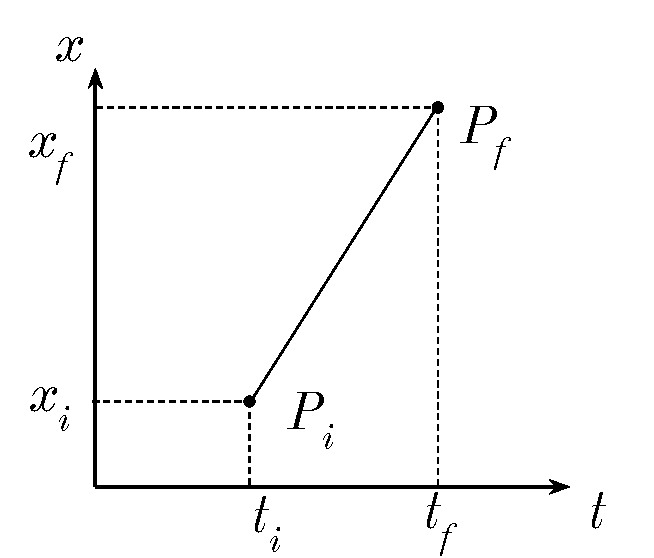
\includegraphics[width = \marginparwidth]{puntomateriale.pdf}
    \caption{Sistema di riferimento con una sola dimensione spaziale ($x$)
    in funzione del tempo ($t$). All'istante $t_i$, il punto materiale $P$
    si trova nella posizione $x_i$}
    \label{point}
\end{marginfigure}

La scelta del sistema di riferimento di assi cartesiani è del tutto arbitraria\footnote{
Gli assi possono addirittura non essere ortogonali, purché si segua la \textit{regola del
parallelogramma} e si rinunci alle proprietà e alle regolarità matematiche degli
assi ortogonali, come il teorema di Pitagora per il calcolo del modulo dei
vettori.}, ma una volta fissata è necessario essere coerenti con essa.
Questo permette di riflettere sul fatto che il moto è sempre relativo al sitema di
riferimento adottato: cambiando sistema di riferimento, il moto cambia.


\subsection{Distanza e spostamento}
Durante il moto, è possibile registrare la \textbf{distanza} percorsa
dall'oggetto e il suo \textbf{spostamento}. Il primo è una grandezza
scalare e corrisponde alla distanza totale percorsa durante il tragitto
effettuato dall'oggetto in moto. Il secondo è una grandezza vettoriale e
corrisponde al cambiamento di posizione,
cioè la differenza tra la posizione iniziale e quella finale dell'oggetto:
\[ \Delta \mathbf{x} = \mathbf{x}_f - \mathbf{x}_i \]


\section{Interpretazioni geometriche}

\begin{marginfigure}
    \centering
    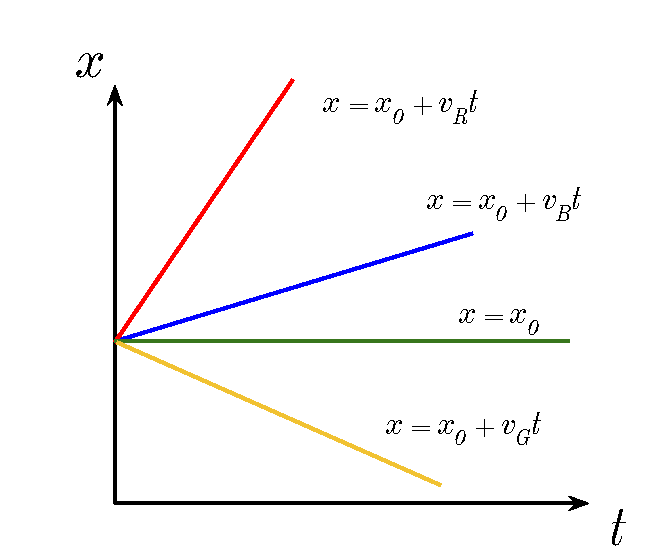
\includegraphics[width = \marginparwidth]{velocita.pdf}
    \caption{Oggetti in moto rettilineo uniforme con velocità differenti}
\end{marginfigure}


\section{Moto rettilineo uniforme}


\section{Accelerazione}



\section{Moto circolare}
Cambiamo ora la traiettoria dell'oggetto in moto, considerando quella circolare.
Per descrivere un moto circolare è conveniente impiegare coordinate differenti,
dette polari. Fissando il centro di un piano cartesiano al centro di una
circonferenza di raggio $r$, possiamo identificare la posizione di ogni punto
della circonferenza con la coppia $(r, \theta)$, dove $\theta$ è l'angolo
formato dalla semiretta appartenente al sistema di riferimento e dalla semiretta
che interseca la circonferenza nel punto desiderato (entrambe le semirette
hanno origine nel centro del piano cartesiano, quindi della circonferenza).

\begin{marginfigure}
    \centering
    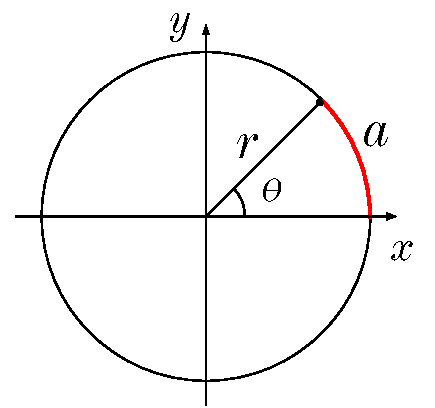
\includegraphics[width = \marginparwidth]{riferimentocirc.pdf}
    \caption{Sistema di riferimento per un moto circolare}
    \label{circref}
\end{marginfigure}

Assumeremo qui che $r$ non varia durante il moto. Per questo, viene omessa
la coordinata $r$ e si considera invece la posizione derivante da $\theta$,
detta anche \textit{posizione angolare}. Convenzionalmente, $\theta > 0$ se
misurato in senso antiorario a partire dall'asse di riferimento (come in
Figura \ref{circref}). Si utilizzano inoltre i \textit{radianti} per misurare
$\theta$. I radianti tornano infatti comodi, perché permettono di semplificare
le relazioni tra le grandezze in gioco durante il moto circolare. Innanzitutto,
dato l'arco $a$ in Figura \ref{circref}, vale la relazione \[ a = r\theta \]
Di fatto, la lunghezza totale della circonferenza corrisponde a $C = 2\pi r$,
dove $2\pi$ corrisponde ad un angolo giro espresso in radianti.

\subsection{Velocità angolare e velocità tangenziale}
Studiamo ora il cambiamento della posizione angolare nel tempo. Come per il
moto rettilineo, possiamo considerare il rapporto tra lo spostamento angolare
e l'intervallo di tempo trascorso. Da qui, si ottiene la velocità angolare:
\[ \omega = \frac{d\theta}{dt} \]
In ogni istante, una particella in moto circolare si muove in direzione
tangenziale alla traiettoria.
\begin{marginfigure}
    \centering
    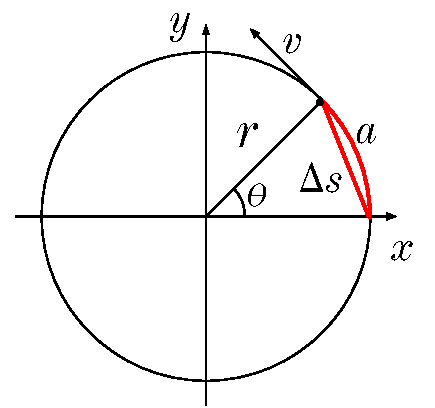
\includegraphics[width = \marginparwidth]{circspeed.pdf}
    \caption{Velocità tangenziale}
    \label{circspeed}
\end{marginfigure}
È chiaro che la particella, muovendosi, copre una certa distanza sulla
circonferenza in un dato intervallo di tempo. Possiamo quindi affermare
che essa ha una velocità, detta \textit{tangenziale}, $v$, oltre che
quella angolare $\omega$. Cerciamo una relazione tra esse: supponiamo che
la particella effettui, in un intervallo infinitesimo $\Delta t$, uno
spostamento angolare altrettanto piccolo $\Delta\theta$ come mostrato in
Figura \ref{circspeed}. Lo spostamento $\Delta s$, dato dalla corda che
sottende l'angolo $\Delta\theta$, approssima l'arco $a = r\Delta\theta$. Quindi:
\[ v = \lim_{\Delta t \to 0}\frac{\Delta s}{\Delta t} = \lim_{\Delta t \to 0} \frac{r\Delta\theta}{\Delta t} = r\lim_{\Delta t \to 0}\frac{\Delta\theta}{\Delta t} = r\omega \]
Abbiamo quindi ottenuto la relazione cercata:
\[ v = r\omega \]
Notare come $v\propto r$, al contrario di $\omega$. Ciò significa che,
assumendo una velocità angolare costante, la velocità tangenziale è tanto
maggiore quanto più $r$ cresce.

\subsection{Moto circolare uniforme}
Un moto circolare uniforme è un moto circolare con velocità \textit{angolare} costante.
Le regolarità di questo tipo di moto permettono di studiare altre grandezze
importanti per il moto circolare: periodi e accelerazioni.

\subsubsection*{Periodo e frequenza}
La particolarità di questo moto è la sua periodicità, perché esso si ripete
ciclicamente nel tempo. In particolare, un oggetto torna ad occupare la medesima
posizione iniziale dopo un certo intervallo di tempo, chiamato \textbf{periodo} ($T$):
in altre parole, il tempo necessario per compiere ``un giro (ciclo) completo''.
Nel nostro caso, un giro completo corrisponde all'intera circonferenza $C = 2\pi$.
Sapendo che $\omega = \frac{d\theta}{dt}$, è immediato ricavare il periodo:
\[ T = \frac{2\pi}{\omega} \]
Si impiega spesso anche la \textbf{frequenza}, che corrisponde al reciproco
del periodo:
\[ f = \frac{1}{T} \]
L'unità di misura è l'\textit{Hertz} (Hz), ovvero ``cicli al secondo'' (s$^{-1}$),
quindi il numero di cicli compiuti nell'unità di tempo.

\subsubsection*{Accelerazione centripeta}
Riprendendo la prima legge della dinamica, sappiamo che un corpo permane nel
suo stato di moto rettilineo uniforme a meno dell'intervento di agenti esterni.
Nel caso dell'intervento di tali agenti, si osserva un'accelerazione
dell'oggetto, ovvero un cambiamento del suo stato di moto e dunque della sua
velocità. Non viene specificato se questo cambiamento avviene al \textit{modulo}
oppure alla \textit{direzione} della velocità. Infatti, la velocità è una
grandezza vettoriale e una variazione di anche una sola delle sue caratteristiche
comporta un'accelerazione. Per questo motivo, nonostante il modulo della velocità
tangenziale di un corpo in moto circolare uniforme sia costante, la direzione
del suo vettore cambia.

Vi è però il problema aperto di trovare l'agente esterno (la forza) che
mantiene l'oggetto (dotato di massa) nella traiettoria del suo moto circolare.
Esso può essere di varia natura: la tensione di una corda attaccata ad una
pallina che viene fatta roteare; la forza di gravitazione universale che
mantiene in orbita (assumiamo circolare) un pianeta intorno ad un sole; la forza
elettrica che mantiene un elettrone vicino al nucleo (secondo un modello classico
dell'atomo).

Vista quindi l'esistenza di un'accelerazione determinata da un agente esterno,
rimane da capire come è fatto il suo vettore (modulo, verso e direzione).
L'esperienza ci dice che questa accelerazione: (1) cresce con l'aumentare della
velocità angolare; (2) è diretta verso il centro della circonferenza. Ma come
dimostrarlo formalmente per tutti i moti circolari uniformi? Consideriamo la
situazione in Figura \ref{circolare}.
\begin{marginfigure}
    \centering
    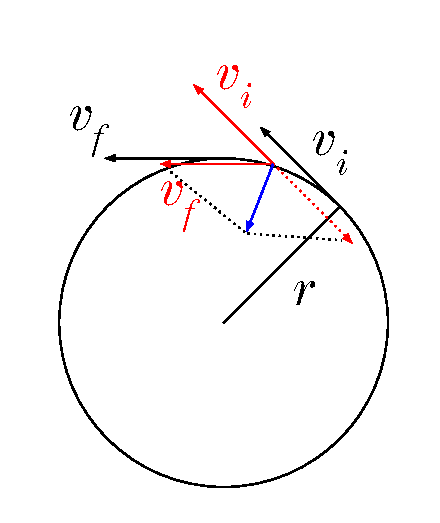
\includegraphics[width = \marginparwidth]{circolare.pdf}
    \caption{Dimostrazione delle caratteristiche geometriche del vettore accelerazione centripeta}
    \label{circolare}
\end{marginfigure}
consideriamo una variazione molto piccola nella posizione angolare dell'oggetto,
che parte con una velocità iniziale $\mathbf{v}_i$ e termina con la
velocità finale $\mathbf{v}_f$, uguali in modulo ma diverse in direzione.
Come già detto, possiamo esprimere l'accelerazione come variazione della
velocità tangenziale.

\[ \mathbf{a} = \frac{d\mathbf{v}}{dt} \simeq \frac{\Delta\mathbf{v}}{\Delta t} \]

\noindent Concentriamoci sul termine $\Delta\mathbf{v}$.

\[ \Delta\mathbf{v} = \mathbf{v}_f - \mathbf{v}_i = \mathbf{v}_f + (-\mathbf{v}_i) \]
Geometricamente, i vettori velocità si sommano secondo la ``regola del parallelogramma''
come mostrato nella Figura. Con i dovuti formalismi geometrici, sapendo che il
modulo di $v$ è sempre costante, possiamo dimostrare che l'accelerazione è
effettivamente centripeta e ortogonale alla velocità tangenziale, ovvero il
suo vettore punta sempre verso il centro della circonferenza. Sempre dalla Figura,
possiamo osservare che al crescere di $v$ cresce anche $a$; tenendo poi
presente che la variazione $\Delta \mathbf{v}$, che è un vettore,
viene moltiplicata per la quantità scalare $\frac{1}{\Delta t}$, il vettore
risultante dell'accelerazione cresce in modulo quanto più piccolo diventa
l'intervallo $\Delta t$: ovvero la velocità dell'oggetto è maggiore.
Dimostreremo più
avanti che la relazione precisa tra i moduli di queste grandezze è data da
\[ a = \frac{v^2}{r} = \omega^2 r \]

\section{Moto armonico}
Supponiamo di osservare un oggetto in moto circolare uniforme, ma invece di
vederlo ``dall'alto'' lo guardiamo con la riconferenza della traiettoria
posta orizzontalmente. Da questo punto di vista, vedremo l'oggetto \textit{oscillare}
a destra e sinistra all'interno di uno spazio la cui larghezza corrisponde al
diametro della circonferenza. Ciò che si vede è un moto particolare, il
\textit{moto armonico semplice}.

Dalla Figura \ref{armonicosemplice} possiamo notare che, fissato il solito
sistema di riferimento $xy$, il moto armonico semplice non è altro che la
proiezione sugli assi di un moto circolare uniforme. Per questo motivo,
possiamo descrivere la posizione dell'oggetto caratterizzato da tale moto:
\begin{marginfigure}
    \centering
    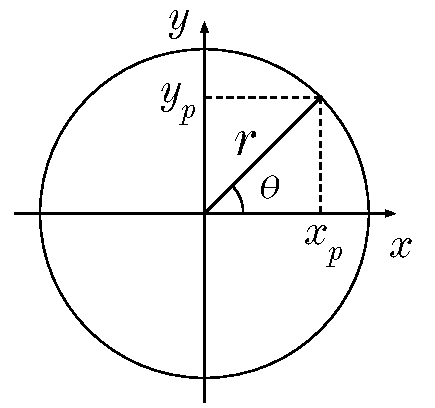
\includegraphics[width = \marginparwidth]{armonico.pdf}
    \caption{Modello di moti armonici semplici a partire da proiezioni
    di un moto circolare uniforme}
    \label{armonicosemplice}
\end{marginfigure}
\[
    \begin{cases}
        x_p(t) = r\cos\theta = r\cos(\omega t)\\
        y_p(t) = r\sin\theta = r\sin(\omega t)
    \end{cases}
\]
Possiamo quindi notare che il moto circolare è la composizione di due moti
armonici.
Sapendo che la velocità corrisponde alla derivata della funzione che
descrive la posizione:
\[
    \begin{cases}
        v_x(t) = -\omega R \sin(\omega t)\\
        v_y(t) = \omega R \cos(\omega t)
    \end{cases}
\]
Derivando nuovamente, otteniamo l'accelerazione:
\[
    \begin{cases}
        a_x(t) = -\omega^2 R\cos(\omega t)\\
        a_y(t) = -\omega^2 R\sin(\omega t)
    \end{cases}
\]
Esiste anche una dimostrazione geometrica di tali relazioni, che non impiega
esplicitamente i metodi del calcolo infinitesimale. È sufficiente tenere in
considerazione la posizione angolare $\theta$, avere dimestichezza con le
funzioni sinusoidali e ricordare direzione e verso dei vettori velocità
tangenziale e accelerazione centripeta durante un moto circolare uniforme.

\subsubsection*{Relazione tra accelerazione centripeta e velocità}
Siamo ora in grado di mostrare l'origine della relazione $a = \frac{v^2}{r} = \omega^2 r$
tra accelerazione centripeta e velocità (angolare e tangenziale) in un moto
circolare uniforme.

Osserviamo che il sistema che descrive l'accelerazione del moto armonico
contiene i termini $r\cos(\omega t)$ e $r\sin(\omega t)$: le coordinate del
punto in moto circolare uniforme in funzione del tempo. Dunque

\[
    \begin{cases}
        a_x(t) = -\omega^2 r\cos(\omega t)\\
        a_y(t) = -\omega^2 r\sin(\omega t)
    \end{cases}
    \Rightarrow
    \begin{cases}
        a_x(t) = -\omega^2 x(t)\\
        a_y(t) = -\omega^2 y(t)
    \end{cases}
\]
Queste non sono altro che le componenti dell'accelerazione centripeta
solidali al sistema di riferimento di assi $xy$. Sapendo che il modulo
di un vettore corrisponde a $|\mathbf{r}| = r = \sqrt{x_r^2 + y_r^2}$
(con $x_r,y_r$ le componenti del vettore $r$ rispetto ad un sistema di
assi ortogonali $xy$), è immediato mostrare che
\[ |\mathbf{a}| = a = \sqrt{(-\omega^2 x)^2 + (-\omega^2 y)^2} = \sqrt{\omega^4x^2 + \omega^4y^2} = \omega^2 \sqrt{x^2 + y^2} = \omega^2 r \]

Dal precedente sistema, è possibile capire perché il vettore dell'accelerazione
è diretto verso il centro della circonferenza: $x$ ed $y$ sono le componenti
del \textit{vettore posizione} dell'oggetto in movimento; tale vettore
non è altro che una freccia di modulo uguale alla lunghezza del raggio e la
cui punta indica il punto in cui il corpo si trova sulla circonferenza,
dunque questo vettore punta verso l'esterno; ma dato che ogni componente
viene moltiplicata per la quantità negativa $-\omega^2$, il vettore
accelerazione centripeta non può che puntare nel verso opposto, quindi
verso il centro della circonferenza. L'equazione vettoriale è dunque la
seguente:
\[ \mathbf{a} = -\frac{\mathbf{v}^2}{\mathbf{r}} \]

\subsubsection*{Accelerazione centripeta, traiettorie curvilinee, raggio di curvatura}
L'accelerazione centripeta non esiste solamente nei moti circolari uniformi,
ma, come possiamo ricordare da esperienze quotidiane, qualsiasi variazione
nella traiettoria di un corpo in moto, attraverso una ``sterzata'', permette
di percepire l'effetto e la direzione dell'accelerazione.
Possiamo dunque estendere la descrizione del moto circolare uniforme a casi
meno eccezionali, come quelli dei moti dalle traiettorie curvilinee. È interessante
come l'equazione dell'accelerazione centripeta permetta di ottenere informazioni
interessantissime su moti come questi, come il \textbf{raggio di curvatura}. Si
osservi l'esempio in Figura \ref{curvilinee}.

\begin{marginfigure}
    \centering
    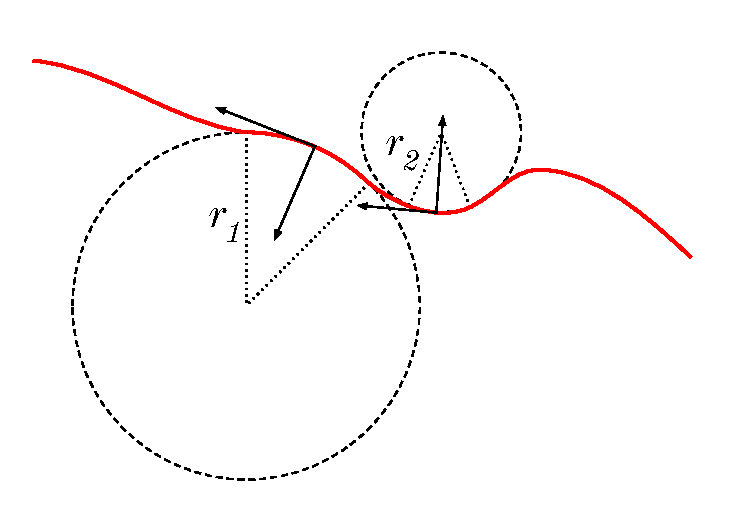
\includegraphics[width = \marginparwidth]{curvilinee.pdf}
    \caption{Una traiettoria curvilinea apporssimata da archi di circonferenze con raggi differenti}
    \label{curvilinee}
\end{marginfigure}

Tratti di traiettorie come queste possono essere approssimate da archi di
circonferenze con raggi di lunghezze differenti. Durante ognuno di questi brevi
tratti, percorsi sugli archi, l'oggetto in moto è sottoposto ad una certa
accelerazione centripeta. Assumento che tale oggetto abbia una massa, è
possibile misurare l'accelerazione rilevando la forza esercitata sull'oggetto
durante il tratto di curva. Dall'equazione dell'accelerazione centripeta,
vale
\[\frac{F}{m} = \frac{v^2}{r}\]
Date le nostre supposizioni sulle grandezze conosciute (forza, massa e velocità), l'unico
dato che rimane è il raggio, che in questo caso prende il nome di
\textit{raggio di curvatura}:
\[ r = \frac{v^2m}{F} \]

\section{Moto nel piano}

\subsubsection*{Parabola di un proiettile}
\[
    \begin{cases}
        x = v_{0,x}t\\
        y = v_{0,y}t - \frac{1}{2}t^2
    \end{cases}
\]
Esprimiamo $y$ in funzione di $x$:
\[
    y = \frac{v_{0,y}}{v_{0,x}}x - \frac{1}{2}\frac{g}{v_{0,x}^2}x^2 = Bx - Cx^2
\]
Tangente a questa parabola:
\[
    y' = B - 2Cx
\]

\subsection{Vettori}
Vettori posizione e spostamento.
\[ \Delta\mathbf{s} = \mathbf{s}_f - \mathbf{s}_i \]

Vettore velocità
\[ \mathbf{v} = \lim_{\Delta t \to 0}\frac{\Delta\mathbf{s}}{\Delta t} = \frac{d\mathbf{s}}{dt} \sim ds\cdot\frac{1}{dt} \]
Per definizione \textit{sempre} tangente alla traiettoria. La traiettoria
è la serie dei punti che si ottiene percorrendo per tratti infinitesimi le
velocità istantanee.

Accelerazione tangente e accelerazione normale.


\subsubsection*{Esercizio}
$|\mathbf{v}_i| = 50\text{ km/h}$, $|\mathbf{v}_f| = 100\text{ km/h}$,
$m = 1800\text{ kg}$, $R = 20\text{ m}$, $\Delta t = 2\text{ s}$. $|\mathbf{F}_n| = ?$ (forza normale),
$|\mathbf{a}_t| = ?$. Assumiamo che l'auto acceleri con costanza tra le
due velocità.

\begin{itemize}
    \item $a_{n,i} = \frac{v_i^2}{R}$, $a_{n,f} = \frac{v_f^2}{R}$
    \item $F_{n,i} = ma_{n,i} \simeq 17100 \text{ N}$, $F_{n,f} = ma_{n,f} \simeq 68400\text{ N}$
    \item $|\mathbf{a}_t| = \textit{cost} = \frac{|\Delta\mathbf{v}|}{\Delta t} \simeq 6,95\text{ m/s}^2$
\end{itemize}


\section*{Recap}
\[ \mathbf{x} = \mathbf{x_0} + \mathbf{v}(t - t_0) \]
Semplificazioni in termini di variazioni, infinità.
% Lezione 3/2024-03-04
% - introduzione alla dinamica
% - prima e seconda legge
% - esercizi su moto uniformemente accelerato
% - accenni al concetto di forza e introduzione alla forza elastica con legge di hooke

% Lezione 4/2024-03-06
% - grafico orario: grafico nel quale un asse riporta lo spazio (una dimensione), mentre sull'altro il tempo
% - differenza tra SPOSTAMENTO e distanza
% - interpretazione grafica della velocità e accelerazione, con analisi di funzione

\chptr{Dinamica}
\marginpar{\minitoc}

\section{Recap}
\[ \overrightarrow{x} = \overrightarrow{x_0} + \overrightarrow{v}(t - t_0) \]
Semplificazioni in termini di variazioni, infinità.

\section{Leggi della dinamica}

Nella descrizione introduttiva del moto, non è stata analizzata alcuna causa del
fenomeno.

\subsection{La prima legge}

\vspace{8pt}
\begin{tcolorbox}[colback = red!30, colframe = red!30!black, title = {Prima legge della dinamica (legge di inerzia)}]
    Un corpo permane nel suo stato di \textit{quiete} o moto rettilineo uniforme
    finché non intervenga un \textit{agente esterno}.
\end{tcolorbox}
\vspace{5pt}

In altre parole, se nulla ``rompe le scatole'' al corpo, esso permanerà nel suo
stato di moto, naturalmente.

\vspace{8pt}
\begin{tcolorbox}[colback = yellow!30, colframe = yellow!30!black, title = {Sistema inerziale}]
    Sistema nel quale vale la prima legge della dinamica.
\end{tcolorbox}
\vspace{5pt}

\subsection{La seconda legge}
Quando l'agente esterno agisce sull'oggetto, l'effetto è un cambiamento nello
stato di moto di quell'oggetto. Ovvero, cambia la sua velocità. La variazione
della velocità nel tempo è chiamata \textbf{accelerazione}.

\[ \lim_{\Delta t \to 0} \frac{\Delta v}{\Delta t} = \frac{dv}{dt} = a \]

\vspace{8pt}
\begin{tcolorbox}[colback = red!30, colframe = red!30!black, title = {Seconda legge della dinamica}]
    \begin{align}
        \frac{|\overrightarrow{F}|}{|\overrightarrow{a}|} = \frac{F}{a} = m
    \end{align}
\end{tcolorbox}
\vspace{5pt}


Gli oggetti hanno inerzia, ovvero capacità di opporsi all'agire dell'agente
esterno. Questa capacità di opporsi è rappresentato da una quantità detta
massa (inerziale).

\subsection{Analisi dimensionale}
\[ [F] = [ma] = \left[m\cdot\frac{v}{t}\right] = \left[m\cdot\frac{l}{t^2}\right]  \]
\[ 1\text{ kg}\cdot\frac{\text{m}}{\text{s}^2} = \text{udm}\left[M\cdot\frac{L}{T^2}\right] = \text{udm}[F] = 1\text{ N} \]


\subsection{Molla e forza elastica}
\[ F \propto \Delta x \]

La forza che la molla esercita, essendo in opposizione alla direzione nella
quale la deformazione viene effettuata, corrisponde a:
\[ F_\textit{el} = -k\Delta x \]

\section{Forza agente sul moto}
Un blocco di massa $m = 10 \text{ kg}$ viaggia ad una velocità $v_i =
2 \text{ m/s}$. Una forza $F = 20 \text{ N}$ agisce sul blocco per
$T = 5 \text{ s}$. Quale velocità raggiungerà il blocco dopo $T$?.
Dopo $T$, la forza cessa di agire e il blocco viaggia a $v_f$ trovata
precedentemente. Includendo lo spazio percorso durante $T$ (e dunque il
tempo $T$), quanto tempo impiega il blocco a coprire $s_w = 2\text{ km}$
di distanza?

\begin{marginfigure}
    \centering
    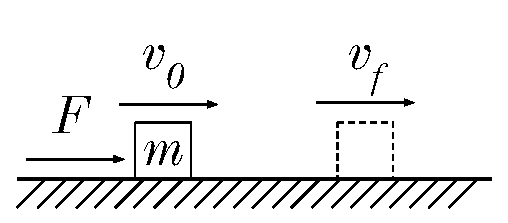
\includegraphics[width = \marginparwidth]{figures/scivola.pdf}
    \caption{Forza agente su una massa in moto}
\end{marginfigure}

Per rispondere al primo quesito, possiamo assumere un moto rettilineo
uniformemente accelerato durante l'intervallo $T$. Sappiamo che \[ a = \frac{F}{m} = \frac{dv}{dt} \]
Da cui possiamo esprimere la velocità in funzione del tempo (la velocità
iniziale la conosciamo già, ma assumiamo un tempo iniziale $t_0 = 0$):
\[ \frac{F}{m}dt = dv \to \int_{t_0}^{t}\frac{F}{m}dp = \int_{v_0}^{v}dw \to \frac{F}{m}\int_{0}^{t}dp = v - v_0 \to \frac{F}{m}t = v - v_0 \]
Dunque
\[ v(t) = v_0 + \frac{F}{m}t \]
Non ci manca che calcolare la velocità in corrispondenza di un $t_f = t_0 + \Delta t = 0 + T = T$:
\[ v(t_f) = v(T) = v_0 + \frac{F}{m}T \]

Nel secondo quesito, possiamo spezzare il problema in due parti: durante
l'azione della forza, la distanza percorsa ($s_a$) deve essere calcolata tenendo
conto del moto uniformemente accelerato, mentre nell'intervallo di tempo
successivo ($T_v$) il moto è semplicemente uniforme. Dalla seguente equazione,
possiamo ricavare $T_v$ ($T$ lo conosciamo già).
\[ s_w = s_a + s_v = s_a + v_fT_v = \int_{0}^{T}(v_0 + at)dp + v_fT_v = v_0T + \frac{1}{2}aT^2 + v_fT_v \]
Il tempo per percorrere $2\text{ km}$ è dunque:
\[ T_{2\text{ km}} = T + \frac{s_w - v_iT - \frac{F}{2m}T^2}{v_f} = T + \frac{s_w - v_iT - \frac{F}{2m}T^2}{v_i + \frac{F}{m}T} \]

\section{Lancio verso l'alto}
Si consideri la situazione mostrata in Figura \ref{lanciobasso}.
Durante la salita, l'oggetto rallenta a causa dell'accelerazione di gravità $g$.
Determiniamo la quota che l'oggetto raggiungerà.

\[ a = \frac{dv}{dt} \to dv = adt \to \int_{v_0}^{v}dw = \int_{t_0}^{t}adp \to v - v_0 = a\int_{t_0}^{t}dp \to v - v_0 = a(t - t_0) \]
Dunque
\[ v(t) = v_0 + a(t - t_0) = v_0 + at \]
Rallentando, si arriverà ad un istante $t_f$ nel quale l'oggetto avrà velocità
nulla:
\begin{marginfigure}
    \centering
    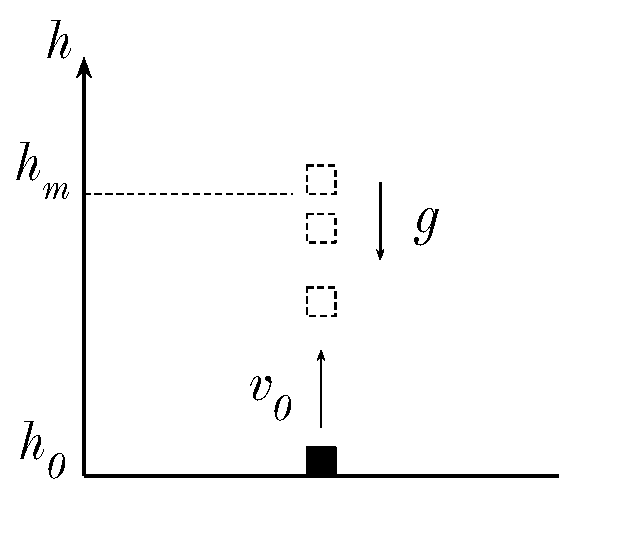
\includegraphics[width = \marginparwidth]{figures/greve.pdf}
    \caption{Lancio di un oggetto verso l'alto}
    \label{lanciobasso}
\end{marginfigure}
\[ v(t_f) = 0 \to v_0 + at_f = 0 \]
Non disponiamo tuttavia del tempo, ma possiamo avvalerci della legge oraria
che descrive la distanza percorsa:
\[ v(t) = \frac{dh}{dt} \to \int_{h_0}^{h}dk = \int_{t_0}^{t}v(t)dp \to h - h_0 = \int_{t_0}^{t}(v_0 + ap)dp \]
\[ h - h_0 = v_0\int_{t_0}^{t}dp + a\int_{t_0}^{t}pdp \to h - h_0 = v_0t + \frac12 at^2 \]
Da cui:
\[ h(t) = h_0 + v_0t + \frac12 at^2 = v_0t + \frac12 at^2 \]
Abbiamo quindi ottenuto la quota in funzione del tempo, che possiamo ricavare
dall'equazione $v_0 + at_f = 0 \to t_f = -\frac{v_0}{a}$.
\[ h(t_f) = v_0t_f + \frac12 at_{f}^2 =  -\frac{v_0^2}{a} + \frac{1}{2}a\frac{v_0^2}{a^2} = -\frac{v_0^2}{a} + \frac{v_0^2}{2a} = -\frac{v_0^2}{2a} \]
Sapendo che $a = -|g|$, la quota massima $h_m$ raggiunta è:
\[ h_m = \frac{v_0^2}{2|g|} \]

%%%%%%%%%%%%%%%%%%%%%%%%%%%%%%%%%%%%%%%%%%%%%%%%%%%%%%%%%%%%%%%%%

\subsection*{Spostamento}
\[ \Delta\overrightarrow{s} = \overrightarrow{s}_f - \overrightarrow{s}_i \]


\subsection{La terza legge}
\vspace{8pt}
\begin{tcolorbox}[colback = red!30, colframe = red!30!black, title = {Terza legge della dinamica}]

\end{tcolorbox}
\vspace{5pt}



\vspace{8pt}
\begin{tcolorbox}[colback = red!30, colframe = red!30!black, title = {Accelerazione centripeta nel moto circolare uniforme}]
\begin{align}
    a = \frac{v^2}{r} = \omega^2 r
\end{align}
\end{tcolorbox}
\vspace{5pt}

\chptr{Meccanica}
\marginpar{\minitoc}

\section{Lavoro di una forza}


Il lavoro di una forza costante corrisponde al prodotto scalare\footnote{Ricordiamo
che il prodotto scalare $p$ tra due vettori \textbf{a} e \textbf{b} è un valore scalare
definito da $p = |\textbf{a}||\textbf{b}|\cos\theta_{\textbf{ab}}$, con $\theta_\textbf{ab}$
l'angolo tra i vettori.}
tra la forza e lo spostamento:
\begin{align}
W = \textbf{F}\cdot\textbf{r}
\end{align}
Il lavoro si misura in Joule (J), dove
\[ 1\text{ J} = 1\text{ Nm} = 1\text{ kg$\frac{\text{m}^2}{\text{s}^2}$} \]


Lavoro di una forza variabile durante lo spostamento:
\begin{align}
    W_{AB} = \int_{A}^{B}\textbf{F}(r)\cdot d\textbf{r}
\end{align}

\section*{app}
Si parte da $\overrightarrow{F} = m\overrightarrow{a} \Rightarrow
\overrightarrow{F} = m\frac{d\overrightarrow{v}}{dt}$. Abbiamo una traiettoria
qualsiasi, posizione descritta da $\overrightarrow{r}(t)$. Prendiamo una variazione
infinitesima della posizione $\Delta\overrightarrow{r}\to d\overrightarrow{r} =
\overrightarrow{r}_f - \overrightarrow{r}_i$.

\subsection{Lavoro di una forza}
\[ dW = \textbf{F}\cdot d\textbf{r} = |\textbf{F}||d\textbf{r}|\cos\theta \]
Può essere positivo, negativo, nullo.
\begin{itemize}
    \item \textbf{Lavoro motore} $dW > 0$
    \item \textbf{Lavoro resistente} $dW < 0$ (la forza si oppone allo spostamento)
    \item \textbf{Lavoro nullo} $dW = 0$ (la forza è ortogonale allo spostamento),
    es forza centripeta
\end{itemize}

Analisi dimensionale:
\[ \left[dW\right] = \left[\textbf{F}d\textbf{r}\right] = \left[M\frac{L}{T^2}L\right] = \left[M\left(\frac{L}{T}\right)^2\right] \]
\[ 1\text{ J} = 1\text{ Nm} = 1\text{ kg$\frac{\text{m}^2}{\text{s}^2}$} \]

Esempio cammino sentiero
\[ W_{A\to B} = \sum_{i = A}^{N = B}dW_i \to \int_{A}^{B}dW \text{ per } N\to\infty \]
\[ W_{A\to B} = \int_{A}^{B}\textbf{F}\cdot d\textbf{r} \]
Notiamo che 
\[ \textbf{P}\cdot d\textbf{r} = |\textbf{P}| (|d\textbf{r}|\cos\theta) \]
Dove abbiamo la proiezione dello spostamento sul peso P. Questo significa che
per calcolo del lavoro importa solo la variazione della quota, $dh$.
\[ W_{0\to 2000\text{ m}} = \sum_{0}^{2000}\textbf{P}\cdot d\textbf{r} = \int_{0}^{2000}mg dh = mgh_{bondone} \]

\subsubsection*{Versore}
\[ \hat{v} = \frac{\overrightarrow{v}}{|\overrightarrow{v}|} \]

\[ W = \int_{i}^{f}\overrightarrow{F}\cdot d\overrightarrow{s} = \int_{0}^{L}(F\hat{f})\cdot(ds\hat{x}) = F(\hat{f}\cdot\hat{x})\int_{0}^{L}ds = F\cos(\theta) L\]
Quindi
\[ \cos\theta = \frac{W}{FL} \]

\section{Teorema delle forze vive}
\textit{vis viva} (forza viva), quantità che viene dalle forze, che pareva avere
vita propria, in grado di trasferirsi da corpo a corpo.
Partiamo da seconda legge della dinamica
\[ \textbf{F} = m\frac{d\textbf{v}}{dt} \]
Senza giustificare le ragioni matematiche dei prossimi passaggi, ma facendoci
guidare dall'intuizione fisica, eseguiamo il prodotto scalare con $d\textbf{s}$
su entrambi i membri
\[ \textbf{F}\cdot d\textbf{s} = m\frac{d\textbf{v}}{dt}\cdot d\textbf{s} = m d\textbf{v}\cdot\frac{d\textbf{s}}{dt} \]
Notiamo che questa operazione ha permesso di ottenere un lavoro al membro di
sinistra, mentre a destra si ottiene il termine $d\mathbf{s}/dt$, che corrisponderebbe
proprio alla velocità $\textbf{v}$. Con ulteriori sviluppi, si raggiunge la
seguente equazione (il simbolo $d$ ha il significato fisico di variazione o
differenza infinitesima).
\[ \textbf{F}\cdot d\textbf{s} = m\textbf{v}\cdot d\textbf{v} = m\text{ }d\left[\frac{v^2}{2}\right] \]
Dimostriamo come sviluppare il termine $\textbf{v}\cdot d\textbf{v} = d\left[\frac{v^2}{2}\right]$.
Ricorriamo alla definizione vettoriale di prodotto scalare\footnote{Il prodotto scalare
di due vettori \textbf{a} e \textbf{b} è calcolabile anche attraverso la somma
dei prodotti tra i valori delle componenti dei due vettori: $\mathbf{a}\cdot\mathbf{b} = a_xb_x + a_yb_y + ...$}
e utilizziamo questo abuso di notazione, ma ragionevole dal punto di vista fisico:
\[ \int x \,dx =  \frac{x^2}{2} + c \Rightarrow \frac{d}{dx}\left[\frac{x^2}{2} + c\right] = x \Rightarrow \int x \,dx = \int d\left[\frac{x^2}{2}\right] \]
Quindi
\[ v_x dv_x + v_y dv_y + v_z dv_z \Rightarrow d\left[\frac{v_x^2}{2}\right] + ... = d\left[\frac{v_x^2 + ...}{2}\right] = d\left[\frac{v^2}{2}\right] \]
Riprendendo l'equazione $\mathbf{F}\cdot d\textbf{s} = m\text{ }d\left[\frac{v^2}{2}\right]$ otteniamo
\[ dW = d\left[\frac12 mv^2\right] \]
Il termine $E_K = \frac{1}{2}mv^2$ viene chiamato \textit{energia cinetica}. Quindi
\[ dW = dE_K \]
Questa equazione può essere tradotta come ``una infinitesima quantità di lavoro
corrisponde ad una variazione infinitesima dell'energia cinetica''. Ora possiamo
enunciare il teorema delle foze vive:
\vspace{8pt}
\begin{tcolorbox}[colback = red!30, colframe = red!30!black, title = {Teorema dell'energia cinetica (o delle forze vive)}]
    Quando una forza (risultante) applicata a un oggetto per un dato tratto di
    traiettoria, compie su di esso un lavoro, il risultato è una variazione del
    modulo della velocità dell'oggetto e quindi una variazione della sua energia
    cinetica. Quindi, il lavoro compiuto su un oggetto è uguale alla variazione
    della sua energia cinetica.
    \begin{align}
        W_{i\to f}^{(R)} = E_{K,f} - E_{K,i}
    \end{align}
\end{tcolorbox}
\vspace{5pt}

\noindent È necessario sottolineare alcune osservazioni:
\begin{enumerate}
    \item Il teorema presuppone che il lavoro sia dovuto all'effetto della risultante delle forze agenti sul corpo.
    \item Il lavoro è rappresentato da una variazione di energia cinetica. Possiamo descrivere dunque lo stato finale
    come \[ E_{K,f} = E_{K,i} + W_{i\to f} \] dunque se il lavoro, quindi l'energia trasferita all'oggetto, è positivo,
    l'energia cinetica aumenta e viceversa.

    \item Il teorema sposta la descrizione del sistema fisico dal piano vettoriale a quello scalare. Ovvero, partendo
    da grandezze vettoriali, abbiamo ottenuto una legge dove compaiono solamente dei numeri. Ciò rende particolarmente agevole
    l'utilizzo del teorema in svariati problemi nei quali l'analisi vettoriale può essere ostica.

    \item Il teorema è molto potente per la sua validità generale, perché non sono state fatte ipotesi sulla natura delle
    forze, se non presupponendo come vera la seconda legge della dinamica $\textbf{F} = m\textbf{a}$.
\end{enumerate}

\subsubsection*{Applicazione del teorema delle forze vive}
Supponiamo di avere un punto di massa $m$ sulla sommità di un piano inclinato di
alteza $h$ con
un angolo $\theta$ rispetto all'orizzontale. Sappiamo che la massa parte dalla
cima con velocità $v_i$ parallela alla lunghezza del piano e diretta verso la
discesa. Vogliamo trovare la velocità finale della massa. Si esprima il calcolo sia
con che senza attrito, considerando nell'ultimo caso un coefficiente di attrito
dinamico $\mu$.
\[ W = \Delta E_K \]
\[ W = \mathbf{P}\cdot\mathbf{L} = |\mathbf{P}||\mathbf{L}|\cos\left(\frac{\pi}{2} - \theta\right) = |\mathbf{P}||\mathbf{L}|\sin\theta = |\mathbf{P}|h = mgh \]
\[ \Delta E_K = \frac12mv_f^2 - \frac12mv_i^2 \]
Quindi
\[ mgh = \frac12mv_f^2 - \frac12mv_i^2 \]
\[ v_f = \sqrt{2gh + v_i^2} \]

Con attrito il peso è contrastato. L'attrito compie il suo lavoro per tutta la
lunghezza del piano fino alla fine della discesa. L'espressione della differenza
di energia cinetica è tuttavia la stessa.
\[ W = W_P - W_A = Ph - F_AL = Ph - \mu F_\perp L = mgh - \mu mg\sin\theta L \]
\chptr{Meccanica degli Urti}
\marginpar{\minitoc}

Fino ad ora abbiamo trattato il moto di corpi ``solitari'', ovvero non
perturbati da altri corpi, ma al massimo influenzati da qualche agente
esterno (le forze). Trattiamo ora gli urti, fenomeni dei quali abbiamo
un'idea intuitiva secondo la quale lo ``scontro'' determina un qualche
cambiamento nella velocità e nella traiettoria degli oggetti coinvolti.
Per trattare gli urti è necessario introdurre due nuove grandezze:
quantità di moto e impulso.


\section{Quantità di moto}
Abbiamo sempre espresso la seconda legge come
\[ \vecsymb{F} = m\vecsymb{a} = m\frac{d\vecsymb{v}}{dt} \]
ma questa proposizione afferma che l'effetto dell'agente esterno (la forza
$\vecsymb{F}$) si traduce interamente in una variazione dello stato di
moto del corpo (accelerazione $\vecsymb{a}$). Si suppone quindi che la
massa sia sempre costante, anche se ciò non è sempre vero. Ad esempio,
un razzo pieno di carburante non avrà la stessa massa che aveva in partenza
una volta arrivato in orbita, quindi la forza esercitata dalla propulsione
dei motori si è tradotta non solo in una variazione dello stato di moto,
ma anche in una variaizione della massa. Non tratteremo sistemi complessi
come il razzo, ma ciò fa intuire che la seconda legge della dinamica può
essere generalizzata nella forma seguente
\begin{align}
    \vecsymb{F} = \frac{d}{dt}(m\vecsymb{v}) = \frac{d\vecsymb{p}}{dt}\label{qtamotosecondalegge}
\end{align}
Dove la quantità $\vecsymb{p}$ prende il nome di \textit{quantià di moto},
definita come
\begin{align}
    \vecsymb{p} \eqdef m\vecsymb{v}
\end{align}
Come dice il termine, la quantità di moto descrive il moto dei corpi
sulla base della velocità di una massa più la massa stessa, a differenza
di quanto accade nello studio cinematico del moto, dove solo le variazioni
dello stato di moto contano, slegate da cause (forze) e materia (massa).
La quantità di moto è inoltre una grandezza vettoriale, perché contiene
in sé la velocità, a sua volta grandezza vettoriale.

%L'effetto della quantità di moto si percepisce in molte situazioni quotidiane.
%Nel bowling, possiamo incassare uno strike perché il moto della palla viene
%trasmesso ai birilli, che a loro volta vengono messi in moto e dunque cadono.
%Se immaginiamo di essere su uno skateboard, in grado di muoversi su un piano
%senza attrito, e chiediamo ad un amico di passarci una palla, è sicuro che
%una volta afferrata la palla lo skateboard sul quale ci troviamo comincerà
%a muoversi. Esso sarà inoltre tan


\section{Impulso}
In molte situazioni comuni le forze agiscono per un tempo brevissimo, come
negli urti. In questi casi è utile introdurre la grandezza dell'impulso.
Supponiamo, ad esempio, che in una partita di baseball il lanciatore faccia
partire la palla a una velocità di 150 km/h. Il battitore ruota il braccio
e colpisce con la mazza la palla, che ritorna verso il lanciatore a 185 km/h.
Nel breve intervallo di tempo durante il quale la palla e la mazza sono in
contatto, dell'ordine del millesimo di secondo, la forza fra esse cresce
rapidamente fino ad un valore massimo molto grande, quindi si annulla quando
la palla si stacca dalla mazza.

Descrivere l'andamento nel tempo della forza che la mazza esercita sulla palla è
difficile. Ciò che possiamo conoscere più facilmente con una strumentazione
adeguata è la \textit{variazione della quantità di moto} (massa e velocità) della
palla a causa del colpo e il tempo $\Delta t$ di contatto tra mazza e palla. Da questi
dati possiamo allora accontentarci di ottenere, usando l'equazione \ref{qtamotosecondalegge} una \textit{forza media}, ovvero
una forza che si è mantenuta costante per tutto l'intervallo di tempo del contatto
mazza-palla.

\[ \left\langle \vecsymb{F}\right\rangle  = \frac{\Delta\vecsymb{p}}{\Delta t} \]

\noindent Riformulando questa equazione per variazioni infinitesime, possiamo
ottenere la variazione di quantità di moto in funzione di $\vecsymb{F}$ e $dt$:

\[ d\vecsymb{p} = \vecsymb{F}dt \]

\noindent Il prodotto $\vecsymb{F}dt$ viene definito \textit{impulso} e non è
altro che una definizione matematica alternativa della variazione della quantità
di moto, utilizzata però più spesso in contesti in cui agiscono forze \textit{impulsive},
cioè forze variabili che agiscono per tempi molto brevi rispetto a quelli
comunemente misurabili nel sistema esaminato.

\begin{align}
    \vecsymb{I} \stackrel{\text{def}}{=} \vecsymb{F}dt
\end{align}

\noindent L'impulso è particolarmente utile per spiegare il motivo per cui
è più confortevole atterrare su 10 metri di neve dopo una caduta di 100 metri
piuttosto che su una lastra di pietra. Per frenare la nostra caduta, la neve
ci permette di sprofondare al suo interno, quindi essa varia la nostra quantità
di moto in maniera graduale e su un intervallo di tempo prolungato. Al contrario,
la lastra di pietra non si deforma in maniera apprezzabile e l'impatto determina
un impulso molto forte rispetto alla neve, tanto da essere letale.


\section{Il fenomeno dell'urto}

\begin{tcolorbox}[colback = yellow!30, colframe = yellow!30!black, title = {Urto}]
    Un urto è un'interazione tra corpi, nella quale si osservano forze
    denominate \textit{impulsive}, che cioè agiscono per tempi e su distanze
    molto più brevi di quelli \textit{tipici} osservabili all'infuori
    dell'urto.
\end{tcolorbox}
\vspace{5pt}

Cosa si intende per distanze e tempi tipici? Per i lettori che ancora si
ricordano, immaginiamo una puntata di Holly \& Benji: Quando i calciatori
si apprestano a sferrare un calcio, il disegnatore sceglie sempre
di rappresentare l'istante del colpo deformando il pallone. Anche se questa
raffigurazione è evidentemente esagerata, essa ha un fondo di verità e offre una spiegazione
intuitiva di cosa si intende per \textit{distanze tipiche dell'urto}: in un
urto, gli oggetti coinvolti si \textit{deformano}. Queste deformazioni avvengono
su distanze ben minori di quelle, per esempio, della traiettoria del calcio o
della lunghezza del campo. In urti reali, inoltre,
come il calcio alla palla di Holly \& Benji, queste deformazioni sono inevitabili,
nonostante i corpi che collidono sembrino apparentemente i più rigidi su
questo pianeta\footnote{Il suono è prova del fatto che sono avvenute vibrazioni
nei corpi, che dunque si sono deformati.}. Bisogna poi specificare che le
deformazioni sono molto difficili da osservare perché, oltre ad avvenire su
distanze ridotte rispetto a quelle tipiche, anche i tempi nelle quali accadono
sono molto brevi. Il contatto tra piede e pallone è molto ridotto rispetto a
quello che invece è richiesto al calciatore per correre dall'angolo al centro
del campo. Riassumendo questo esempio calcistico, quando osserviamo una
partita siamo di fronte a grandezze \textit{tipiche} (dimensioni del campo da
calcio, velocità dei calciatori e della palla, ecc.); negli urti, invece,
possiamo trascurare le deformazioni e le distanze, perché troppo piccole
rispetto a quelle tipiche, e i tempi, perché gli urti appaiono come eventi
istantanei ai nostri occhi.

L'intenzione della meccanica di questo capitolo, dunque, non è quella di
descrivere ciò che accade \textit{durante} l'urto, ma prevedere, date le
informazioni \textit{precedenti} all'urto, lo stato del sistema
\textit{successivamente} all'urto. Idealmente, l'urto avviene istantaneamente
e i corpi coinvolti sono sempre punti materiali, che dunque non conoscono
deformazioni.

\subsection*{Urti e quantità di moto}
Vogliamo prevedere lo stato del sistema dopo l'urto, in termini di
velocità (vettori) dei corpi coinvolti. Sorprendentemente, gli unici
strumenti che servono per trattare in modo semplice questo problema
sono i tre principi della dinamica, più la definizione di quantità
di moto e l'assunzione del \textit{sistema isolato}, ovvero non
disturbato da forze esterne.

Un classico esempio che unisce nozioni su urti e quantità di moto è il
tavolo da biliardo. Supponiamo di avere due palle, 1 e 2, sul tavolo in moto
rettilineo
uniforme e in rotta di collisione tra loro; ovvero, sappiamo con certezza
che la loro traiettoria si intersecherà e che tale punto verrà raggiunto
da entrambi i corpi nel medesimo istante di tempo. L'esprerienza ci permette
di concludere che, passata la \textit{zona d'urto}, le palle non procederanno
sulle stesse rette dei moti precedenti, ma devieranno.
Dobbiamo fare alcune assunzioni fondamentali. Innanzitutto, supporremo che
nessun altro agente agirà sul sistema appena descritto (aiuterebbe immaginare
due palle che vagano nello spazio profondo, o in altre parole: Nulla deve
disturbare il sistema).
Immaginiamo l'intervallo temporale nel quale le due palle saranno a contatto
tra loro, collidendo: entrambe eserciteranno una forza sull'altra e aiutati
dalla terza legge della dinamica sappiamo che

\[ \vecsymb{F}_{1 \to 2} = -\vecsymb{F}_{2 \to 1} \]

\noindent cioè l'applicazione di una forza su una palla determina una forza identica
in modulo e direzione, ma verso opposto e applicata sull'altra palla.
Sviluppiamo l'equazione sfruttando la definizione di quantità di moto,
ricordando che una forza $x \to y$ determina una variazione dello stato di
moto di $y$.
\[ \frac{d\vecsymb{p}_2}{dt} = -\frac{d\vecsymb{p}_1}{dt} \]
Ricorrendo agli usuali abusi di notazione matematica, ma ragionevoli da
un punto di vista fisico, semplifichiamo l'intervallo di tempo infinitesimale
del differenziale:
\begin{align*}
    &d\vecsymb{p}_2 = -d\vecsymb{p}_1\\
    &d[\vecsymb{p}_1 + \vecsymb{p}_2] = 0\\
    &d\vecsymb{p}_\text{tot} = 0
\end{align*}
Abbiamo mostrato, in anticipo, che per un sistema di due corpi come le palle
da biliardo, assumendo che non agiscano forze esterne, la quantità di moto
totale del sistema si conserva. Come l'energia meccanica, possiamo dunque
concludere che un urto ideale non modifichi la quantità di moto del sistema.
Questa conclusione è ancora incompleta e inesatta perché, come scopriremo
in una prossima sezione, la quantità di moto si conserva \textit{sempre} in
un sistema isolato e non dipende dalla natura dell'urto.

\section{Conservazione}
Come l'energia, nella storia della fisica si è sempre pensasto al moto
come una quantità che potesse essere trasferita da un corpo ad un altro,
fatto ragionevole ben giustificato dall'esperienza: basti pensare al
gioco del biliardo.
Come già dedusse Cartesio, la ``macchina dell'universo'', assimilata ad
un orologio, non può continuare a funzionare senza che una qualche quantità
si conservi. Egli stesso fu tra i primi a proporre il prodotto massa-velocità
come misura di tale quantità: due carri identici che viaggiano a velocità differenti
hanno chiaramente quantità di moto diverse, ma una palla di cannone
racchiude in sé maggior moto rispetto ad un sasso lanciato alla stessa
velocità. Queste quantità sono presenti negli oggetti secondo distribuzioni
differenti e variabili nel tempo, ma nel complesso esse non possono che
sommarsi (vettorialmente!) sempre nella medesima quantità; se l'universo è un
sistema chiuso, e lo si può supporre per definizione, allora la quantità di moto
non può sparire o comparire, ma può trasferirsi tra gli oggetti al suo
interno, trasformarsi.

\subsection{Forze interne ed esterne}
Approfondiamo il concetto di \textit{sistema di punti materiali} e studiamone
uno contentente un certo numero di punti materiali $N$. Immaginiamo che
tra questi punti agiscano forze di varia natura: repulsive elettriche,
attrattive gravitazionali ecc.; inoltre, supponiamo che vengano applicate
altre forze dall'esterno di questo sistema di punti materiali\footnote{Una
immagine esplicativa è il polmone, dove le molecole dell'aria formano i
punti materiali e i muscoli del torace sono gli agenti esterni.}.
Possiamo suddividere le forze in gioco in due insiemi:
\begin{enumerate}
    \item \textbf{Forze interne}: le forze che i punti esercitano gli uni
    sugli altri. Forze che descrivono l'interazione tra i punti.
    \item \textbf{Forze esterne}: le forze che l'ambiente esterno esercita
    sul sistema, l'insieme di punti.
\end{enumerate}
Ogni punto $i$-esimo sarà sottoposto ad una certa forza totale, o risultante, derivante
dalla somma/sovrapposizione di tutte le forze precedentemente descritte
\begin{align*}
    \vecsymb{R}_i = m_i\vecsymb{a}_i\\
    \vecsymb{R}^{(E)}_i + \vecsymb{R}^{(I)}_i = m_i\vecsymb{a}_i
\end{align*}
Definiamo le risultanti delle forze esterne, ed interne agenti sul punto
$i$-esimo:
\begin{align*}
    \vecsymb{R}^{(E)}_i &\eqdef \sum_{k} \vecsymb{F}^{(E)}_{k \to i}\\
    \vecsymb{R}^{(I)}_i &\eqdef \sum_{j} \vecsymb{F}^{(I)}_{j \to i} \qquad j \not = i
\end{align*}
Supponiamo che un punto non eserciti alcuna forza su se stesso (per questo
poniamo $i \not = j$).
La risultante di tutte le forze in gioco sarà
\[ \vecsymb{R} = \sum_{i} \vecsymb{R}_i \]
In tale somma, concentriamoci sulla risultante delle forze interne:
\[ \vecsymb{R}^{(I)} = \sum_{i} \vecsymb{R}^{(I)}_i = \sum_{i} \sum_{j} \vecsymb{F}^{(I)}_{j \to i} \]
In questa somma, supponiamo che non vi siano forze agenti su un corpo
ed esercitate dal corpo stesso, dunque poniamo $\vecsymb{F}^{(I)}_{j \to i} = \overrightarrow{0} \quad \forall j = i$.
Sappiamo che vale la terza legge della dinamica, dunque
$\vecsymb{F}^{(I)}_{j \to i} = -\vecsymb{F}^{(I)}_{i \to j}$. Ma allora
\begin{align}
    \vecsymb{R}^{(I)} = \sum_{i} \sum_{j} \vecsymb{F}^{(I)}_{j \to i} = \overrightarrow{0}\label{interne}
\end{align}
Abbiamo appena dimostrato, grazie all'ipotesi della terza legge,
che, in un sistema di punti materiali, la risultante delle forze interne
è nulla.

\subsection{Centro di massa}
Dall'Equazione \ref{interne} possiamo dedurre che la risultante delle
forze, interne ed esterne, coinvolte in un sistema di punti materiali
è determinata solamente dalle forze esterne.
\[ \vecsymb{R} = \vecsymb{R}^{(E)} = \sum_{i} \vecsymb{R}^{(E)}_i = \sum_i m_i\vecsymb{a}_i \]
Dalla precedente equazione, si può ricavare un'interessante definizione:
\[ \sum_i m_i\vecsymb{a}_i = \sum_i m_i \frac{d^2\vecsymb{x}_i}{dt^2} = \left(\sum_i m_i\right) \frac{d^2}{dt^2}\left[ \frac{\sum_i m_i\vecsymb{x}_i}{\sum_i m_i} \right] \]
Abbiamo ottenuto un termine molto interessante, un artificio matematico
che ha interpretazioni e applicazioni piuttosto importanti: \textit{il
centro di massa}.
\begin{align}
    \vecsymb{x}_\text{CM} \eqdef \frac{\sum_i m_i\vecsymb{x}_i}{\sum_i m_i}
\end{align}
Dalla definizione è banane\footnote{Esattamente, banane. Ci scusiamo per questo scherzo di nevrosi.} ricavare la velocità e l'accelerazione del
centro di massa. Riprendendo le equazioni precedenti e ponendo $M = \sum_i m_i$,
possiamo concludere che
\[ \vecsymb{R}^{(E)} = M\frac{d^2\vecsymb{x}_\text{CM}}{dt^2} = M\vecsymb{a}_\text{CM} \]

\subsection{La legge di conservazione della quantità di moto}
In un sistema isolato, non si rilevano forze esterne. Allora
\[ \vecsymb{R}^{(E)} = \overrightarrow{0} \quad \therefore \quad M\vecsymb{a}_\text{CM} = 0 \quad \therefore \quad \vecsymb{a}_\text{CM} = 0 \]
ovvero, la velocità del centro di massa è costante, quindi la
quantità di moto del centro di massa è costante e si conserva in
un sistema isolato. Vale dunque la seguente in un sistema isolato:

\begin{align*}
    \vecsymb{v}_{\text{CM}, i} &= \vecsymb{v}_{\text{CM}, f}\\
    \frac{\sum_j m_j\vecsymb{v}_{j,i}}{M} &= \frac{\sum_j m_j\vecsymb{v}_{j,f}}{M}\\
    \vecsymb{p}_{\text{tot}, i} &= \vecsymb{p}_{\text{tot}, f}
\end{align*}

\noindent Da cui

\begin{align}
    \frac{d}{dt}\vecsymb{p}_\text{tot} = 0
\end{align}
Tale risultato ha conseguenze di portata non trascurabile. Si consideri
infatti il problema esposto nella prossima sottosezione.

\subsubsection*{Punto di collisione}
Due magneti di massa $m$ e $5m$ sono mantenuti ad una distanza fissa tra
di loro. Una volta rimossi i vincoli, i due magneti si attraggono fino a
schiantarsi. Sapendo che il primo magnete si trovava in posizione $x_1 = 0$
mentre il secondo in $x_2 = 8\text{ cm}$, si intende individuare la posizione
della collisione.

Alla luce della legge di conservazione della quantità di moto, sappiamo
che nella situazione iniziale la quantità di moto totale del sistema è
nulla, in quanto i due magneti sono mantenuti fermi.
\[ \vecsymb{p}_i = 0 \]
Il problema non fa alcun cenno all'azione di forze esterne, dunque possiamo
supporre che il sistema sia isolato e che dunque la quantità di moto
iniziale si conserverà anche subito prima dell'urto. Vale allora:
\[ \vecsymb{p}_i = m\vecsymb{v}_{i,\text{tot}} = 0 \Rightarrow \vecsymb{v}_{i,\text{tot}} = 0 \]
Ma sappiamo anche che la velocità totale è rappresentato dal centro di massa
del sistema. Ciò significa che se il centro di massa era ``fermo''
inizialmente, rimarrà tale anche poco prima dell'urto, grazie alla legge
di conservazione della quantità di moto. Basta dunque trovare la posizione
del centro di massa e il gioco è fatto.
\[ x_\text{CM} = \frac{mx_1 + 5mx_2}{m + 5m} = \frac{x_1 + 5x_2}{6} = \frac{5}{6}x_2 \]


\section{Impulso}
\[ \left\langle \vecsymb{F} \right\rangle = \vecsymb{F}_\text{impulsiva} \simeq \frac{\Delta\vecsymb{p}}{\Delta t} \]
\[ \Delta\vecsymb{p} = \vecsymb{F}_\text{impulsiva}\Delta t \]
Deformazioni per tempi brevi, tempo di contatto.
\[ \Delta\vecsymb{p} = m\vecsymb{v}_f - m(\overrightarrow{0}) \qquad F_\text{imp} = \frac{mv_f}{T} \]


\section{Urti elastici}
\begin{tcolorbox}[colback = yellow!30, colframe = yellow!30!black, title = {Urto}]
    In un urto elastico, si conservano la quantità di moto e l'energia cinetica.
\end{tcolorbox}
\vspace{5pt}

\noindent Un sistema contenente un certo numero di corpi può dunque essere descritto come segue:
\begin{align}
    \begin{cases}
        \sum_j m_j\vecsymb{v}_{0,j} = \sum_j m_j\vecsymb{v}_{f,j} \qquad \text{conservazione della quantità di moto}\\
        \sum_j m_j\vecsymb{v}_{0,j}^2 = \sum_j m_j\vecsymb{v}_{f,j}^2 \qquad \text{conservazione dell'energia cinetica}
    \end{cases}
\end{align}
Nella realtà comunemente osservabile, urti pressoché elasti avvengono tra
oggetti che rimbalzano tra loro dopo un urto, anche se in realtà l'energia
cinetica viene inevitabilmente dissipata in altre forme (suono e calore), rendendo
l'urto stesso non del tutto elastico. Sono idealmente elastici urti tra
particelle, a livello molecolare e atomico\footnote{Questa assunzione sarà fondamentale
nella teoria cinetica dei gas}.

\section{Urti anelastici}
\begin{tcolorbox}[colback = yellow!30, colframe = yellow!30!black, title = {Urto}]
    In un urto anelastico, la quantità di moto del sistema si conserva, mentre
    l'energia cinetica totale no.
\end{tcolorbox}
\vspace{5pt}

\noindent Negli urti anelastici, vale sempre la legge di conservazione della quantità
di moto. Tutti gli urti reali sono anelastici e un esempio di \textit{urto perfettamente
anelastico} è quello di due corpi che rimangono uniti dopo l'urto. Supponiamo di avere due masse che viaggiano ad una certa velocità
e in rotta di collisione tra loro. Dopo l'urto, le due masse rimangono
in contatto. Supponendo che le due masse attaccate formino un unico corpo, Vale:

\[ \vecsymb{p}_{1,i} + \vecsymb{p}_{2,i} = \vecsymb{p}_{3,f} \]

\noindent Dal punto di vista energetico, però, accade qualcosa di strano. Osserviamo
l'energia cinetica:

\[ E_{K,i} = E_{K1, i} + E_{K2, i} = \frac12 m_1\vecsymb{v}_{1,i}^2 + \frac12 m_2\vecsymb{v}_{2,i}^2\]

\noindent Supponiamo di porre gli oggetti nel sistema di riferimento del centro di massa
e di osservare esternamente la situazione (poniamo $\vecsymb{v} = \vecsymb{v}_\text{CM} + \vecsymb{v}_\text{scm}$):

\[ E_{K,i} = \frac12 m_1(\textbf{v}_\text{CM} + \vecsymb{v}_{1,i,\text{scm}})^2 + \frac12 m_2(\textbf{v}_\text{CM} + \vecsymb{v}_{2,i,\text{scm}})^2 = \frac12(m_1 + m_2)\vecsymb{v}_\text{CM}^2 + E'_{K,i} \]

\noindent dove abbiamo isolato i termini nei quali compare la velocità del centro di massa
elevata al quadrato, per poi condensare l'energia rimanente in $E'_{K,i}$,
la cui forma non è per noi rilevante. Se invece calcoliamo l'energia cinetica
finale,
\[ E_{K,f} = \frac12 (m_1 + m_2)\vecsymb{v}_{3,f}^2 = \frac12(m_1 + m_2)\vecsymb{v}_\text{CM}^2 \]
è immediato infatti notare che, data la conservazione della quantità di moto,
il corpo finale comprensivo di entrambe le massse non potrà che muoversi
con velocità identica a quella del centro di massa.
Abbiamo dunque mostrato che in generale l'energia cinetica non si conserva nell'urto.
In particolare, essa diminuisce sempre in situazioni reali.

\begin{align}
    E_{K,f} \leq E_{K,i}
\end{align}

\noindent Il motivo di tale fenomeno può essere spiegato attraverso numerose
interpretazioni, che possono dipendere dal sistema analizzato. In generale,
la perdita di energia cinetica è dovuta al costo per mantenere unite le
masse dopo l'urto, oppure, come accade sempre nella realtà, quell'energia
viene dissipata in calore, deformazioni permanenti dei materiali, suono e
così via.

\section{Il pendolo balistico}
\chptr{Relatività del Moto}
\marginpar{\minitoc}

\epigraph{\emph{``That view of things would be normal for me if I normally walked on my hands.''}}{\href{https://www.youtube.com/watch?v=bJMYoj4hHqU}{\textcolor{blue}{\textit{Frames of Reference (1960) - Hume, Ivey\footnotemark[1]}}}}\footnote{Chiedo aiuto, sto impazzendo: Ditemi che il volto all'istante 2:27 non è quello del professor Casari...}

Cominciamo questo capitolo ponendo al lettore una domanda:

\begin{center}
    \textit{Sei aristotelica/o oppure copernicana/o?}
\end{center}

\noindent Senza soffermarci troppo su cosa essa intenda,
sottolineamo brevemente che ciò di cui si tratta in questo capitolo
è stato uno dei temi più controversi nella storia della fisica, quello
che forse ha sconvolto di più convinzioni un tempo ben radicate e
che ha infiammato dibattiti che hanno pure fatto la storia della
letteratura\footnote{\href{https://youtu.be/0kxarmulkiA?feature=shared&t=6180}{\textcolor{blue}{\textit{Marco Paolini - ITIS Galileo}}} (circa 10 minuti a partire dal tempo 1:43:00).}. E non è tutto qui: Gli ultimi grandi sviluppi della relatività
del moto sono avvenuti poco più di un secolo fa ad opera di Einstein
e molti altri e i cambiamenti da loro apportati hanno condotto a
stravolgimenti ancora più bizzarri. Perché ciò che questo ramo della
fisica rivela è che più osserviamo con attenzione la realtà, più essa non
è come un attimo prima poteva sembrare. Per tale motivo la relatività può
essere allo stesso tempo semplice e complessa, perché offre una visione
del tutto insolita di ciò che ci appare come ``normale''.


\section{Sistemi di riferimento}
``Relativo'' è un termine che ben si sposa con l'espressione ``a qualcosa''.
Quel qualcosa viene definito nelle teorie relativistiche della fisica
\textit{sistema di riferimento}, che intuitivamente rappresenta il punto di
vista dal quale si effettuano delle misurazioni o semplici osservazioni di
fenomeni. Ricordiamo che tra le coordinate di un sistema di riferimento
è presente anche il tempo.

\begin{tcolorbox}[colback = yellow!30, colframe = yellow!30!black, title = {Sistema di riferimento}]
    Un insieme di strumenti geometrico-algebrici, di coordinate solidali con un
    oggetto arbitrario, e di procedure che consentono di individuare la posizione
    di un punto di uno spazio metrico.
\end{tcolorbox}

Una volta fissato il sistema di riferimento, tutte le misurazioni devono
essere coerenti con esso, se si intende adottare quel punto di vista.
Quando diciamo che un'auto viaggia a 110 km/h, stiamo in realtà fornendo
un'informazione incompleta, perché sottintendiamo che tale misurazione
sia stata effettuata rispetto alla strada. Non potremmo dire la stessa
cosa se viaggiassimo su un'altra auto che affianca la prima, con stessa
direzione e verso: Diremmo che
l'auto che prima, vista dalla strada, si muoveva a 110 km/h ora sta viaggiando con velocità
minore rispetto a noi. Il moto di un corpo è sempre relativo a un sistema di riferimento.
Cambiando il sistema, il moto cambia. Vedremo nei prossimi paragrafi
che però non tutti i sistemi di riferimento sono uguali e possono
distinguersi in \textit{inerziali} e \textit{non inerziali}.

Il cambiamento riguarda anche le traiettorie: Se lanciassimo una pallina
verso l'alto mentre viaggiamo sulla carrozza di un treno con velocità
costante, vedremmo la pallina salire e scendere su una linea retta.
Un osservatore esterno, invece vedrebbe la pallina muoversi secondo
una traiettoria parabolica. Vedremo che i moti si compongono
ed è necessario effettuare trasformazioni tra le coordinate dei
sistemi di riferimento.

\section{Principio di relatività galileiana}

\begin{tcolorbox}[colback = yellow!30, colframe = yellow!30!black, title = {Principio dei relatività galileiana}]
Le leggi della dinamica newtoniana hanno la stessa forma in tutti i
sistemi di riferimento inerziali.

In relazione alle proprietà cinematiche di un punto materiale, il legame
tra un sistema di riferimento inerziale, con origine $o$, e un altro
sistema di riferimento inerziale, con origine $o'$, è descritta dalla
seguente trasformazione:

\begin{align}
\begin{cases}
    \vecsymb{r} = \vecsymb{r}' + \vecsymb{oo}'\\
    \vecsymb{v} = \vecsymb{v}' + \vecsymb{v}_{o'}
\end{cases}
\end{align}
\end{tcolorbox}


\section{Forze apparenti}


\subsection{L'ascensore}

%\section{Approfondimento: RR}
%Questa sezione è interamente dedicata alla relatività ristretta, sviluppata
%nelle sue forme più celebri da Einstein nei primi lustri del Ventesimo secolo.
%Vogliamo dare un assaggio di questa teoria per vari motivi: Si tratta in primo
%luogo di fisica classica (gli strumenti matematici impiegati sono pressoché gli stessi); essa è inoltre un buon esempio di ridefinizione e affinamento
%radicali di teorie precedenti, innanzitutto la relatività galileiana, e convinzioni
%comuni.

%\subsection{I principi della relatività ristretta}
\chptr{Gravitazione}
\marginpar{\minitoc}

\section{Gravità e forze fondamentali}
Conosciamo bene la seconda legge della dinamica $\mathbf{F} = m\mathbf{a}$.
Sappiamo che il termine $\mathbf{F}$ rappresenta l'azione di un agente esterno,
chiamato forza, che può avere natura diversa a seconda del sistema studiato.
Pertanto, possiamo esprimere
la sua intensità in forme a volte diverse, sia essa il peso, l'attrito, la
forza elastica e così via. Tuttavia tutte queste forze, per quanto sappiamo al
giorno d'oggi, sono riconducibili a quattro interazioni fondamentali che si
manifestano nella materia (dalla più forte alla più debole):
\begin{itemize}
    \item \textit{Forza forte}: la più forte tra tutte. Tiene insieme i nuclei
    degli atomi.

    \item \textit{Forza elettromagnetica}: accoppia le cariche elettriche e
    le correnti.

    \item \textit{Forza debole}: si manifesta in fenomeni di decadimento nucleare.
    
    \item \textit{Forza gravitazionale}: la più debole tra tutte.
\end{itemize}
Lo stato attuale della fisica suggerisce che molte di queste forze possano essere
unificate, ovvero esse non sono altro che la manifestazione, in nature differenti,
della stessa forza fondamentale.
Sorprendentemente, è stata la forza più debole ad essere studiata per prima.
La legge fondamentale venne formulata da Newton nel seguente modo:

\begin{align}
    \mathbf{F}_{\text{G}, 1\to 2} = -G\frac{m_{\text{G},1}m_{\text{G},2}}{r^2_{1,2}}\hat{r}_{1,2}\label{gravity}
\end{align}

\noindent Che esprime il vettore della forza gravitazionale che un corpo 1 esercita su un
altro corpo 2. Il vettore giace sulla congiungente tra i due corpi (considerati come
punti materiali), separati da una distanza $r_{1,2}$ e dotati di una certa
\textit{massa gravitazionale} $m_G$. Il segno negativo, accompagnato dalla
\textit{costante di gravitazione universale}, indica che la forza gravitazionale è
sempre attrattiva.

\section{Il principio di equivalenza}
Soffermiamoci a chiarire alcuni concetti. Innanzitutto, vogliamo esprimere la legge
\ref{gravity} in maniera più generica.

\begin{align}
    \mathbf{F} = c\frac{p_1p_2}{r^2}\hat{r} \label{template}
\end{align}

\noindent Sorprendentemente, questa forma verrà proposta da Coulomb per esprimere
l'interazione tra due cariche elettriche, secondo la legge (in moduli)

\[ F_E = k\frac{|q_1||q_2|}{r^2} \]

\noindent Diventa naturale pensare che la \ref{template} possa rappresentare una
sorta di ``template'' con il quale esprimere quantitativamente l'interazione tra due
oggetti dotati di una certa qualità o proprietà intrinseca $p$, che consente agli oggetti in
questione di partecipare nell'interazione. Nel caso delle cariche elettriche,
essa sarà, per l'appunto, una carica elettrica. Per quanto riguarda la gravità,
questa qualità è la massa gravitazionale. Ci si può chiedere se stiamo parlando
della stessa massa della seconda legge di Newton. In realtà, esse sono ben diverse:
\begin{itemize}
    \item La massa inerziale $m_I$ esprime la capacità di un corpo di opporsi all'azione
    di agenti esterni e, di conseguenza, al cambiamento del proprio stato di moto.
    In breve, essa misura l'inerzia del corpo.

    \item La massa gravitazionale $m_G$ esprime la capacità di un corpo di partecipare,
    contribuire ed essere soggetto all'interazione gravitazionale in presenza di
    un altro corpo dotato di massa gravitazionale.
\end{itemize}
Seppur sottile, la differenza tra queste quantità è
comunque diversa (un oggetto ``massivo'' è difficile da spostare; un oggetto ``massiccio''
interagisce maggiormente con un altro oggetto). La parola ``carica'' sarebbe più intuitiva per spiegare la differenza
e viene infatti utilizzata per le interazioni elettriche: più ``carico'' di una certa
proprietà dell'interazione, più ``intensa'' l'interazione stessa. Nella pratica ci
riferiamo sempre alla stessa massa (i kilogrammi), ma nulla impedisce di pensare che le masse di
uno stesso corpo siano effettivamente quantità distinte.

Consideriamo un corpo in prossimità della superficie terrestre. Possiamo approssimare
la Terra ad una sfera uniforme e supporre che la forza gravitazionale corpo-Terra
giaccia sulla congiungente tra il centro del pianeta e il corpo (puntiforme). Il
corpo si trova ad una certa altezza $h$ e conosciamo inoltre il raggio della Terra
$R_T$. Il corpò sarà soggetto alla forza gravitazionale della Terra; uniamo le
equazioni di Newton (consideriamo i moduli):
\[ F = m_\text{I,C}a \qquad F = G\frac{m_\text{G,C}M_\text{G,T}}{(R_{T} + h)^2} \]
Supponiamo che $R_T \gg h$. Dunque la distanza Terra-corpo può essere approssimata:
\[ r_\text{T,C} = R_T + h = R_T\left(1 + \frac{h}{R_T}\right) \]
\[ r_\text{T,C}^2 \simeq R_T^2\left( 1 + 2\frac{h}{R_T} \right) \]
\[ \frac{1}{r_\text{T,C}^2} \simeq \frac{1}{R_T^2}\left( 1 - 2\frac{h}{R_T} \right) \]

\noindent Da cui concludiamo che possiamo trascurare $h$. Dunque, sapendo che
$a = g$,

\[ m_\text{I,C}g = G\frac{m_\text{G,C}M_\text{G,T}}{R_{T}^2} \]

\noindent Isoliamo $g$

\[ g = \frac{m_\text{G,C}}{m_\text{I,C}}G\frac{M_\text{G,T}}{R_{T}^2} \]

\noindent Se assumessimo che le masse inerziale e gravitazionale di uno stesso corpo
fossero diverse, l'accelerazione $g$ non sarebbe la stessa per tutti gli oggetti. Tuttavia,
non è ancora stata trovata evidenza della differenza quantitativa (apprezzabile, in
quanto misure sperimentali) tra le due proprietà. L'osservazione galileiana stessa
sulla caduta libera, ovvero che tutti i corpi cadono con la stessa accelerazione,
indica che

\begin{align}
    m_I = m_G
\end{align}

\noindent che rappresenta il principio di equivalenza tra massa inerziale e massa
gravitazionale. Possiamo affermare ciò perché,
fisttata la massa della Terra e il suo raggio,
il rapporto $m_I/m_G$ deve essere costante
affinché $g$ sia uguale per tutti i corpi di massa distinta.

\section{Approfondimenti}

\subsection{Energia potenziale gravitazionale}
Si usa spesso calcolare l'energia potenziale di un oggetto vicino alla superficie
terrestre, ad un'altitudine $h$, con la seguente legge:

\[ mgh \]

\noindent Tuttavia sappiamo che $g$ non è costante al variare della quota e su grandi
distanze questa legge non è più una buona approssimazione. Calcoliamo dunque la differenza
di energia potenziale tra la superficie terrestre e una certa quota $h$ da essa alla luce
della legge di Newton.

\[ \Delta\mathcal{U} = -W = -\int_{R}^{R + h}-G\frac{mM}{s^2}\,ds = GmM\int_{R}^{R+h}\frac{ds}{s^2} = GmM\left[ -\frac{1}{s} \right]_{R}^{R+h} =  \]
\[ = -GmM\left( \frac{1}{R + h} - \frac{1}{R} \right) \]

\noindent Notiamo che $\Delta\mathcal{U} > 0$, dunque allontanando un oggetto di massa
$m$ dalla superficie terrestre, esso guadagna una certa energia potenziale. Più in generale,
se poniamo un punto di riferimento $X$ arbitrario dal quale calcolare la (differenza di)
energia potenziale verso un punto $P$, otteniamo la seguente espressione:

\[ \mathcal{U}(P) = -GmM\left(\frac{1}{r_P} - \frac{1}{r_X}\right) \]

\noindent Per convenienza è utile porre $r_X = +\infty$, ovvero ad una distanza infinita da
$M$, ottenendo dunque

\[ \mathcal{U} = -\frac{GmM}{r} \]

\noindent L'energia meccanica di un corpo è dunque

\[ E = E_K + \mathcal{U} = \frac{1}{2}mv^2 -\frac{GmM}{r} \]

\noindent Ovviamente supponiamo che tutte queste leggi valgano per punti materiali.
In un caso reale, per esempio per il calcolo dell'energia potenziale gravitazionale
in prossimità della Terra, quando si ``sprofonda'' nel corpo che genera il campo
gravitazionale, l'estensione di tale corpo modifica l'andamento dell'energia potenziale.

\subsection{Gravitazione universale}
Secondo la legge di Newton, tutti gli oggetti nell'universo si attraggono l'un l'altro
attraverso l'interazione gravitazionale. è in questo senso che la legge viene detta
``universale''.

\subsubsection*{La terza legge di Keplero}
Ovviamente la legge di Newton ha grande importanza in campo astronomico (anche
se espressa in forme assai più complesse) ed è stata la conferma di una legge scoperta
sperimentalmente tempo addietro da Keplero, appunto la \textit{terza legge di Keplero}:

\[ T \propto r^\frac{3}{2} \]

\noindent Secondo tale legge, il periodo $T$ di rivoluzione di un pianeta attorno al Sole
è proporzionale alla distanza media $r$ del pianeta dal Sole elevata a $3/2$. Dunque esiste
una costante $k$ tale che $T = kr^\frac{3}{2}$. In realtà
questa legge vale per tutti i sistemi astronomici (solari e non) simili al nostro, ma
gli studi di Keplero si basavano sugli attenti dati raccolti dal maestro Tycho Brahe
sui moti orbitali dei corpi celesti appartenenti al sistema solare.
Sapendo infatti che la forza di gravità tra un pianeta e il Sole è proprio la forza
centripeta del moto orbitale, assunto come circolare, dimostrare la terza legge di
Keplero diventa ovvio:

\[ T = \frac{2\pi}{\omega} = \frac{2\pi}{v}r = \frac{2\pi}{\sqrt{a_c r}}r = \frac{2\pi}{\sqrt{\frac{GM}{r}}}r = \left(\frac{2\pi}{\sqrt{GM}}\right)r^\frac{3}{2} \]

\noindent Non solo abbiamo dimostrato la terza legge, ma abbiamo pure individuato la
costante di proporizonalità $k$.

\subsubsection*{Sistemi binari}
Dedichiamo questa sezione ad un classico problema di gravitazione piuttosto complesso,
ma altrettanto interessante, presente peraltro in natura nonostante il classico
modello copernicano al quale siamo abituati.

In sistemi non simili a quello solare vale ancora la legge di Newton. Consideriamo
per esempio un sistema di stelle binarie, ovvero stelle con una differenza di massa
non trascurabile rispetto alla distanza del centro di massa del sistema dal centro
di massa di una delle due stelle. In tale caso, le stelle orbiteranno attorno al
loro centro di massa, situato in qualche punto dello spazio intermedio sulla loro
congiungente. Anche nel sistema solare la Terra e il Sole ruotano attorno al centro
di massa totale, che tuttavia si trova ben al di sotto della superficie del Sole,
il che permette di ridurre la trattazione del problema ad una rivoluzione della
Terra attorno al Sole.
\chptr{Termodimaica}

\section{Introduzione}
D'ora in poi, il ruolo dell'energia sarà ancora più importante. In precedenza
abbiamo dimostrato che la differenza di energia meccanica di un corpo corrisponde
al lavoro totale delle forze non conservative.

\[ W^\text{NC} = \Delta E \]

\noindent In altri termini, l'energia che un corpo possiede viene persa o acquistata
nel caso in cui vi siano forze non conservative che compiano lavoro effettivo. Ma
quindi l'unico modo di ``parlare'', ovvero scambiare energia, con l'universo è quello
di compiere lavoro? In realtà no, come vedremo parlando di \textit{calore}, la forma
di energia più ``disordinata'' che conosciamo.

Ci occuperemo di sistemi contenenti un numero di costituenti nell'ordine di

\[ N_A = 6 \cdot 10^{23} \]

\noindent ossia il numero di Avogadro. Questi costituenti possono scambiare energia
attraverso ciò che definiremo calore.

\subsection*{Sistemi termodinamici}
Le nostre trattazioni avranno per oggetto i \textit{sistemi termodinamici}, per
definizione contenuto in un \textit{ambiente esterno}. Ambiente esterno e il suo
contenuto costituiscono l'\textit{universo}, per definizione l'unico sistema che
non è contenuto in un altro ambiente esterno.
Altro oggetto di nostro interesse per lo studio di questi sistemi sono le
\textit{trasformazioni termodinamiche}, ovvero processi nei quali avvengono
scambi di energia.

Possiamo classificare i sistemi termodinamici sulla base di due criteri: capacità
di scambiare materia e capacità di scambiare energia.

\subsection*{Variabili termodinamiche}
In cinematica utilizziamo variabili spazio-temporali per descrivere i nostri
sistemi di punti materiali. Fare questo per un numero di punti o costituenti
dell'ordine di $10^{23}$ è di fatto proibitivo. In termodinamica si utilizzano
invece grandezze diverse, dette \textit{variabili (o coordinate) termodinamiche}.
Le distinguiamo in

\begin{itemize}
    \item \textbf{Grandezze intensive}: si possono misurare localmente,
    indipendentemente dall'estensione dell'oggetto che ne è caratterizzato.
    Sono grandezze intensive la \textit{pressione} e la \textit{temperatura}.

    \item \textbf{Grandezze estensive}: è necessario considerare l'oggetto nel
    suo complesso, non ha senso o non si può misurare in un punto locale arbitrario.
    Sono grandezze estensive il \textit{volume} e la \textit{massa}.
\end{itemize}

\noindent Come in cinematica impiegavamo un sistema di assi cartesiani come
forma di rappresentazione del sistema di punti materiali in moto nelle dimensioni,
anche in termodinamica utilizziamo il medesimo strumento, ma utilizzando le
coordinate termodinamiche. Una trasformazione termodinamica consiste in uno
spostamento tra due punti $A$ e $B$ su questo nuovo piano cartesiano e assumeremo
sempre, affinché la nostra teoria funzioni, che $A$ e $B$ siano situazioni, stati, di
\textit{equilibrio termodinamico}. Nel mezzo non vi è garanzia di equilibrio.

Un sistema si dice in equilibrio dinamico se esso rispetta i seguenti equilibri:
\begin{enumerate}
    \item \textbf{Equilibrio meccanico}: lo stato non è sottoposto a forze totali non nulle,
    in qualsiasi coppia delle sue parti.

    \item \textbf{Equilibrio chimico}: non esiste alcuna reazione chimica tra una qualsiasi
    coppia di parti dello stato.

    \item \textbf{Equilibrio termico}: per ogni coppia di parti, la temperatura è la stessa.
\end{enumerate}

\noindent Per ``parti'' di uno stato o di un sistema intendiamo sottoinsiemi
abbastanza piccoli rispetto al sistema originale ma allo stesso tempo sufficientemente
grandi affiché gli strumenti della termodinamica funzionino.

\section{Calore e scambi}
\section{Gas ideali}
\subsection{Leggi dei gas ideali}
\subsection{Lavoro di un gas ideale}

\section{La teoria cinetica dei gas}
Finora abbiamo affrontato la termodinamica parlando spesso di gas.
Lo abbiamo fatto inoltre da un punto di vista macroscopico, ovvero
utilizzando variabili termodinamiche (pressione, volume, temperatura).
Tuttavia, vogliamo ora tentare di costruire un modello che permetta
di spiegare cosa accade a livello microscopico e che sia allo stesso
tempo coerente con le leggi mostrate fino ad ora.
Per giungere a tale obbiettivo, ovvero collegare macroscopico e mocroscopico,
l'unico strumento che abbiamo a diposizione in questo corso è la meccanica.
Questa è la via che porta alla cosiddetta \textit{teoria cinetica dei
gas}.

\subsection*{Ipotesi e presupposti della teoria cinetica}
La teoria cinetica dei gas semplifica molto ciò che veramente accade
nella realtà fisica, ma è una approssimazione piuttosto buona e
soddisfacente. In particolare, chiariamo che la teoria si basa sulle
seguenti ipotesi:
\begin{itemize}
    \item Oggetto delle osservazioni è un gas \textit{ideale} (o
    perfetto) che si trova all'interno di un contenitore con volume
    $V$.

    \item Il gas è ideale nel senso che esso è costituito da
    particelle infinitamente piccole rispetto al contenitore nel
    quale sitrovano e alle distanze che le separano; tali particelle
    sono inoltre tutte uguali, compresa massa e altre proprietà.

    \item Il gas ha una densità bassa nell'ordine in cui le interazione
    tra le sue particelle è minimo o possibilmente nullo (non avvengono
    urti, interazioni gravitazionali o di qualsiasi altra natura).

    \item Gli unici urti di interesse teorico, non trascurabili, sono
    quelli con le pareti del contenitore, perfettamente elastici (la
    massa delle particelle è infinitamente piccola rispetto a quella
    delle pareti del contenitore).
\end{itemize}

\subsection*{Logica della teoria}
Per semplificare i calcoli, supponiamo che il contenitore sia un
cubo con lati di lunghezza $L$. Si consideri una sola particella
di gas (massa $m$) che sta per urtare la parete destra e la componente $x$
della sua velocità ($v_x$). La quantità di moto iniziale di tale particella
è

\[ \mathbf{p}_{x,i} = m\textbf{v}_{x,i} \]

Avviene un urto elastico con la parete destra, dunque la velocità finale
della particella è uguale in modulo a quella iniziale, ma con verso
opposto:

\[ \mathbf{p}_{x,f} = m\textbf{v}_{x,f} = -m\textbf{v}_{x,i} \]

La variazione della quantità di moto della particella equivale dunque
a

\[ \Delta\mathbf{p}_x = -2mv_x\hat{x} \]

Utilizziamo d'ora in poi i moduli dei vettori. Sappiamo che tale
variazione nella quantità di moto della particella può essere
interpretata come un impulso esercitato dalla parete; dunque la
parete esercita una forza sulla particella, ma come calcolarla?
Diventa necessario trovare un intervallo temporale entro il quale
agisce l'impulso per ricavare l'intensita della forza.
Semplicemente notiamo che la velocità della particella non varia,
per via degli urti elastici, e dunque essa rimbalza ripetutamente
a destra e sinistra nel cubo. Dunque, la particella impiega un tempo

\[ \Delta t = \frac{2L}{v_x} \]

Per lasciare la parete e tornarvici per un altro urto. In media nel
tempo, dunque, la forza impulsiva esercitata dalla parete destra
sulla particella equivale a

\[ F_x = \left|\frac{\Delta p_x}{\Delta t}\right| = 2mv_x \cdot \frac{v_x}{2L} = \frac{mv_x^2}{L} \]

Dalla definizione di pressione, otteniamo la pressione esercitata
dalla particella che rimbalza tra due pareti opposte (di superficie
$S = L^2$):

\[ p_x = \frac{F_x}{S} = \frac{mv_x^2}{L^3} = \frac{mv_x^2}{V} \]

Lo stesso ragionamento vale per tutte le componenti spaziali.
Macroscopicamente, osserviamo che la pressione è una quantità intensiva,
che non dipende dalla località della misurazione. Dunque tutte
le dimensioni spaziali sono equivalenti e possiamo effettuare la
seguente semplificazione:

\[ p_x = p_y = p_z = p \]

Unendo la legge dei gas perfetti al risultato ottenuto precedentemente,

\[ pV = mv_x^2 \]

Ma ciò riguarda solamente una singola particella. Sommiamo dunque
tutti i contributi:

\[ F_{\text{tot}, x} = \sum_i F_{x,i} = \sum_i \frac{mv_{x,i}^2}{L} = \frac{m}{L}\sum_iv_{x,i}^2 \]

In generale le velocità delle particelle potrebbero non essere tutte
uguali. Supponendo che il gas sia costituito da $N$ particelle, possiamo
determinare la loro velocità quadratica media

\[ F_{\text{tot},x} = N\frac{m}{L}\overline{v_x^2} \]

Dunque

\[ pV = Nm\overline{v_x^2} \]

Sappiamo che $v^2 = v_x^2 + v_y^2 + v_z^2$, che vale anche per la
velocità quadratica media $\overline{v^2}$. Ma trattando delle medie,
i contributi di tutte le dimensioni sono tra loro equivalenti:

\[ \overline{v_x^2} = \overline{v_y^2} = \overline{v_z^2} \]

Da cui

\[ \overline{v^2} = \overline{v_x^2} + \overline{v_y^2} + \overline{v_z^2} = 3\overline{v_x^2} \]

Allora

\[ pV = Nm\frac{\overline{v^2}}{3} = \frac{2}{3}N\overline{E_K}\]

Dove abbiamo esplicitato l'energia cinetica media della singola particella.
Per andare più in profondità, possiamo notare che la teoria può
portarci a concludere che

\[ N\overline{E_K} = E_{int} = U \]

Abbiamo dunque collegato la nostra teoria da un lato e gli esperimenti
dall'altro:

\[ pV = Nk_BT = \frac{2}{3}U \]

Possiamo inoltre osservare dalla precedente che

\[ \overline{E_K} = \frac{3}{2}k_BT \]

Che esprime la relazione tra energia cinetica media di una particella
e la temperatura. In un certo senso, dunque, la temperatura \textit{è}
proprio l'energia cinetica media delle particelle.

\subsection*{Risultati della teroria}
Il risultato più importante della teoria cinetica è l'unione tra
il mondo macroscopico osservato sperimentalmente e il mondo microscopico
modellato teoricamente. In particolare:
\begin{itemize}
    \item La teoria cinetica offre una spiegazione dell'origine della
    pressione esercitata da un gas in un contenitore.

    \item La teoria cinetica mostra che la temperatura è strettamente
    legata all'energia cinetica media delle particelle. Intuitivamente,
    la temperatura è interpretabile proprio come l'agitazione media
    delle particelle, per l'appunto l'energia del loro movimento.

    \item La teoria cinetica costruisce un modello generalizzabile
    a sistemi di costituenti non necessariamente monoatomico-puntiformi,
    come approfondito nella prossima sezione.
\end{itemize}

\subsubsection*{Gradi di libertà}
Il fattore $1/2$ deriva dalla definizione di enrgia cinetica, ma
il numero $3$ invece? Esso dipende dal numero di dimensioni entro
le quali le particelle possono muoversi, ovvero i \textit{gradi di
libertà}. Se compissimo lo studio da capo, costringendo però le particelle
a giacere su un piano, i gradi di libertà sarebbero solo due e il fattore
moltiplicativo
dell'energia cinetica media sarebbe diverso. Ciò è dovuto al fatto
che ogni grado di libertà permette alla particella di muoversi su
un'altra dimensione e dunque di aggiungere un contributo in più alla
propria energia cinetica. In generale, dunque, ogni grado di
liberta comporta un contributo energetico di $\frac12k_BT$ e
dunque, per $l$ gradi di libertà, si ottiene

\[ \overline{E_K} = \frac{l}{2}k_BT \]

I gradi di libertà possono crescere all'aumentare della complessità
della particella di gas. Oltre alle tre dimensioni, una molecola
biatomica (quindi non puntiforme come abbiamo sempre supposto finora)
può anche ruotare su due assi\footnote{Due assi sono sufficienti a
coprire tutte le rotazioni nelle tre dimensioni}; i due atomi possono
poi vibrare intorno alla loro ``sede'' nella molecola, dunque anche
questa energia deve essere presa in considerazione. In totale, una
molecola biatomica ideale può avere $l = 6$ gradi di libertà.


\section{Trasformazioni termodinamiche}
Abbiamo mostrato che il lavoro di un gas ideale (ovvero a bassa densità)
è legato al volume e alla temperatura dalla seguente relazione:

\[ W_{A\to B} = \int_{A,\gamma}^{B}p(V)dV \]

\noindent Notare che è sempre necessario specificare il ``percorso'' $\gamma$
che il gas intraprende nel piano pressione-volume (e temperatura),
perchè in generale il lavoro dipende da tale percorso. Ricordiamo
infatti che

\[ \Delta U = Q - W \quad\text{ ma }\quad dU = \delta Q - \delta W \]

\noindent dove $\delta$ indica una quantità dipendente dai punti attraversati.
La differenza finale $dU$ sarà sempre la stessa, ma può derivare
da contributi differenti di calore e lavoro. Nelle prossime sezioni
sostituiremo $\delta$ con $d$, perché ci limiteremo a definire una
sola trasformazione alla volta, quindi un solo tratto di percorso
ben definito. L'equazione $dU = \delta Q - \delta W$ è più generale
perché presuppone la possibilità che il gas possa compiere più di una
trasformazione per variare la propria energia interna.

Il ``percorso'' prende il nome di \textit{trasformazione termodinamica}
e studieremo ora le più semplici. Ricordiamo inoltre che le
trasformazioni che verranno mostrate sono \textit{quasistatiche}
e che quindi ogni punto può essere approssimato ad uno stato di
equilibrio differente.

\subsection{Trasformazione isocora}
Nelle trasformazioni isocore, il volume del gas rimane costante.
Segue dunque

\[ dV = 0 \Rightarrow dW = pdV = 0 \Rightarrow dU = dQ \]

\noindent Sappiamo dagli studi di calorimetria che possiamo associare al
gas un certo calore specifico $c_v$ che permette di descrivere il calore
scambiato rispetto alla variazione di temperatura. Utilizziamo per
convenienza un calore specifico \textit{molare}, anziché ricorrere
alla massa. Bisogna però specificare che tale calore specifico
vale solo a volume costante.

\[ dQ = nc_VdT \]

Da cui

\[ dU = nc_VdT \]
Dal momento che l'energia interna di un gas dipende solamente dalla
temperatura, ciò vale anche per la sua variazione. Dunque, anche
nelle trasformazioni che vedremo di seguito possiamo supporre che
valga tale relazione.

Dalla teoria cinetica abbiamo inoltre osservato che l'energia
interna di un gas equivale a $U = \frac32nRT$, da cui
$dU = \frac32nRdT$
Possiamo dunque concludere con la seguente proposizione (per i
gas ideali monoatomici):

\[ c_V = \frac{3}{2}R \]

\noindent In generale, avendo $l$ gradi di libertà vale $c_V = \frac{l}{2}R$.

\subsection{Trasformazione isobara}
Per una trasformazione isobara, la pressione rimane costante.
Diventa dunque facile calcolare il lavoro effettuato in tale
trasformazione:

\[ W_\text{isobara} = p\Delta V = nR\Delta T \]

\noindent Dalle trasformazioni isocore abbiamo concluso che $dU = nc_VdT$.
Per quanto riguarda il calore, dobbiamo introdurre un ulteriore
calore specifico $c_p$ che invece vale per trasformazioni isobare.

\[ dQ = nc_pdT \]

\noindent Riproponiamo l'equazione di stato dei gas ideali $pV = nRT$ e
consideriamo una variazione infinitesimale su entrambi i membri.

\[ d[pV] = d[nRT] \]
\[ dpV + pdV = nRdT \]
\[ pdV = dW = nRdT \]

\noindent Dunque $dU = nc_pdT - nRdT = nc_vdT$, da cui la seguente relazione.

\begin{align}
    c_p - c_v = R
\end{align}

\noindent Quella che abbiamo appena ottenuto è la cosiddetta \textit{relazione
di Mayer} (esatto, lo studentato). Dai risultati precedenti otteniamo

\[ c_p = c_v + R = \frac52R \]

Se riformuliamo la relazione di Mayer otteniamo una ulteriore relazione
molto impiegata nello studio di un'altra trasformazione che vedremo.

\[ R = c_V\left(\frac{c_p}{c_V} - 1\right) = c_V(\gamma - 1) > 0 \]

\noindent Incontreremo di nuovo il rapporto $\gamma$. Da questo risultato
risulta dunque che

\[ c_p > c_V \]

\noindent sempre (entro il nostro modello). Ma come mai è importante precisare
questa osservazione? In verità tale relazione ha un riscontro reale
e sperimentale: in una trasformazione isocora, il volume non varia;
d'altra parte in trasformazioni isobare la pressione viene mantenuta
costante e ciò significa che il gas deve esercitare tale pressione
costante durante tutal la trasformazione. Ciò comporta la necessità di un
supplemento di energia dovuto alla variazione di volume e alla costanza
della pressione. Di fatto, per aumentare l'energia interna di un
gas è necessario fornire maggior energia qualora la pressione rimanga
costante (per esempio in un contenitore chiuso da uno stantuffo mobile,
dove il gas impiega energie per sollevare lo stantuffo), mentre risulta
meno dispendioso innalzare l'energia interna di un gas a volume
costante. Da qui il motivo della disuguaglianza $c_p > c_V$.

\subsection{Trasformazioni isoterme}
Nelle trasformazioni isoterme, la temperatura non varia. Come
conseguenza, nemmeno l'energia interna varia.

\[ dU = nc_VdT = 0 \]

Segue dunque che

\[ dQ - dW = 0 \]
\[ dQ = dW = pdV = nRT\frac{dV}{V} \]
\[ Q_\text{isoterma} = \int_{i}^{f}nRT\frac{dV}{V} = nRT\ln\left(\frac{V_f}{V_i}\right) = W_\text{isoterma} \]

In una isoterma, dunque, non varia l'energia interna, perché il calore
scambiato viene ``consumato'' in una quantità uguale di lavoro.

\subsection{Trasformazioni adiabatiche}
In queste trasformazioni non avvengono scambi di calore.

\[ dU = dQ - dW = -dW \]

Come sempre, sapendo che la variazione di energia interna è esprimibile
attraverso una corrispondente variazione di temperatura legata a $c_V$,

\[ nc_VdT = -pdV \]

\[ nc_VdT = -nRTdV \]

Otteniamo dunque la seguente relazione:

\[ \frac{dT}{T} = -\frac{R}{c_V}\frac{dV}{V} \]

\[ \int_{i}^{f}\frac{dT}{T} = -\frac{R}{c_V}\int_{i}^{f}\frac{dV}{V} \]

\[ \ln\left( \frac{T_f}{T_i} \right) = -(\gamma - 1)\ln\left(\frac{V_f}{V_i}\right) \]

\[ T_i V_i^{\gamma - 1} = T_fV_f^{\gamma - 1} \]

Vale allora per le adiabatiche

\begin{align}
    TV^{\gamma - 1} = \text{const}\\
    pV^\gamma = \text{const}
\end{align}

In particolare, nel caso di trasformazioni adiabatiche che coinvolgono
gas monotatomici risulta $pV^{\frac53} = \text{const}$.

\subsection{Esercizio: trasformazioni cicliche}


\section{Macchine}

%\setcounter{chapter}{0}

\part*{Appendici}
\appendix
\renewcommand{\thechapter}{\Alph{chapter}}
\chptr{Esercizi}

\section{Effetto centrifuga}

Un corpo è vincolato a muoversi lungo una guida
rigida (può muoversi parallelamente alla guida
ma non perpendicolarmente ad essa) che sta
ruotando intorno ad uno dei suoi estremi con
velocità angolare $\omega$ (rad/s). Inizialmente
il corpo si trova a $d_0$ m dall'asse di rotazione
ed è fermo; dopo un certo intervallo di tempo
il corpo ha raggiunto una posizione $d_f$ (m)
ed ha una velocità $v_f$ (m/s). Dati
$d_0 = 1$, $d_f = 2.5$, $v_f = 8.1$, trovare
$\omega$.
\begin{enumerate}
    \item 5.0
    \item 5.6
    \item 8.9
    \item 3.5
\end{enumerate}

\noindent \textbf{Soluzione:}
Fissiamo un sistema di riferimento
solidale con la guida. In tal modo, è come se
l'oggetto si stesse muovendo solamente in linea
retta sulla guida stessa. In tale situazione,
l'oggetto si sposta verso l'esterno per via
della forza centrifuga, una forza apparente,
perché il sistema di riferimento scelto
non è inerziale.

Ricorriamo ad una analisi energetica. L'energia
cinetica dell'oggetto viene incrementata dall'azione
della forza centrifuga; ciò suggerisce il ricorso
al teorema dell'energia cinetica:

\begin{align}
    \Delta E_K &= W_{F_c}\label{g1}\\
    K_f - K_0 &= \int_{d_0}^{d_f}F_c ds\label{g2}\\
    \frac12 m v_f^2 &= \int_{d_0}^{d_f}m\omega^2sds\label{g3}\\
    v_f^2 &= \omega^2(d_f^2 - d_0^2)\label{g4}
\end{align}

\noindent da cui il risultato cercato

\[ \omega = \frac{v_f}{\sqrt{d_f^2 - d_0^2}} \]

\noindent Eseguendo i calcoli, risulta che la risposta
(4) è quella corretta. Analizziamo più chiaramente i passaggi:
In \ref{g1} esprimiamo il teorema delle forze vive
come variazione dell'energia cinetica dell'oggetto
equivalente al lavoro compiuto dalla forza centrifuga $F_c$.
In \ref{g2} esplicitiamo la differenza tra le energie
cinetiche iniziale e finale; dall'altro membro costruiamo
invece l'integrale che permette di ottenere il lavoro
totale dalla posizione iniziale $d_0$ a $d_f$: ricorriamo
alla definizione più generale di lavoro (appunto impiegando
il calcolo integrale), perché $F_c$ varia durante il
percorso da $d_0$ a $d_f$. In \ref{g3} possiamo accorgerci
che l'energia cinetica iniziale è nulla (il testo afferma
che l'oggetto è inizialmente fermo rispetto alla guida);
al membro di destra esprimiamo invece $F_c$ in funzione
di $m$, $\omega$ e $s$, dove $s$ rappresenta la posizione
dell'oggetto a partire dal fulcro sul quale ruota la guida.
Per ricavare questa relazione
abbiamo utilizzato la definizione di forza centripeta
(che si rivela essere, in modulo, la stessa di quella
centrifuga)

\[ a_c = \omega^2 s \]

\noindent In \ref{g4} cancelliamo i termini comuni
come la massa e il fattore $\frac12$ (che compare
anche al membro di destra per via dell'integrazione
del tipo $\int xdx = x^2/2$). Notiamo poi che $\omega$
è costante, perché la guida ruota con velocità angolare
costante, e può essere ``estratto'' dall'integrale.

\noindent \textbf{Nozioni chiave:} moto circolare uniforme, sistemi
di riferimento non inerziali, energia meccanica.


\section{Rincorsa sul cuneo}
Una massa $m$ (kg) si muove inizialmente su un piano
orizzontale privo di attrito con velocità $v_0$ (m/s).
Successivamente essa sale su un piano inclinato, inizialmente
fermo rispetto al piano orizzontale, di
massa $M$ (kg), che consiste in un cuneo libero di
muoversi anch'esso sul piano. La velocità $v_0$ è
tale che $m$ si ferma esattamente sulla sommità del
cuneo, ad altezza $h$ (cm). Si supponga che non vi
siano attriti di alcun genere. Dati $m = 11.0$, $M = 47.0$
e $h = 25.0$, trovare $v_0$.

\begin{enumerate}
    \item 4.1
    \item 8.5
    \item 2.5
    \item 6.0
\end{enumerate}

\noindent \textbf{Soluzione:}


\section{\textit{Raindrops are falling on my head}}
Una goccia di pioggia di raggio $R$ (mm)
cade da una nuvola. Durante la caduta
questa risente della resistenza aerodinamica
opposta dall'aria che possiamo modellizzare
come $F = \frac12 D \rho_\text{aria} S v^2$,
dove $D$ è il coefficiente aerodinamico,
$S$ la superficie d'impatto della goccia e
$v$ la sua velocità. Si assuma la goccia
sferica e le densità di aria e acqua pari a
$\rho_\text{aria} = 1.2$ kg/m$^3$ e
$\rho_\text{H$_2$O} = 1000$ kg/m$^3$. Sotto
queste assunzioni la velocità limite della
goccia cresce fino a stabilizzarsi al
valore limite $v_f$ (m/s). Dati $D = 0.78$,
$v_f = 24.0$, trovare $R$.

\begin{enumerate}
    \item 40.4
    \item 28.1
    \item 59.2
    \item 20.6
\end{enumerate}

\noindent \textbf{Soluzione:}

\section{Valuta l'offerta}
Vostro cugino Nunzio vi dice che ha inventato una macchina termica che assorbe
calore da una fonte a 30°C e cede calore ad un pozzo a 15°C. Secondo Nunzio
l'efficienza della macchina è pari al 15\%. La comprereste?

\noindent \textbf{Soluzione:}
\chptr{Leggi fisiche notevoli}

\section{Legge di Hooke}
La legge di Hooke è una legge empirica che pone in relazione la forza
di richiamo esercitata da una molla e l'estensione della deformazione
che genera quella stessa forza.

\begin{align}
    \vecsymb{F} = -k \Delta\vecsymb{x}\label{hooke}
\end{align}

\noindent Si suppone che la deformazione $\Delta\vecsymb{x}$ avvenga sulla
stessa retta sulla quale la molla giace.


\section{Legge di Stefan-Boltzmann}

\begin{align}
    \varepsilon = \sigma e T^4\label{stefanboltzmann}
\end{align}

\section{Legge di Newton gravitazione universale}


\begin{align}
    \vecsymb{F} = -G \frac{m M}{\vecsymb{r}^2}\hat{r}
\end{align}

\section{Legge di Avogadro}

\begin{align}
    N = \frac{1}{k_B} \frac{pV}{T}
\end{align}

\section{Legge di Boyle}
\begin{align}
    p \propto \frac{1}{V}
\end{align}

\section{Equazione armonica}

\begin{align}
    \frac{d^2\vecsymb{x}}{dt^2} + \omega^2\vecsymb{x} = 0\label{harmony}
\end{align}

\section{Oscillatore a molla}

\begin{align}
    T = 2\pi \sqrt{\frac{m}{k}}
\end{align}

\section{Pendolo}

\begin{align}
    T = 2\pi \sqrt{\frac{l}{g}}
\end{align}
\chptr{Costanti}

\vspace*{0.5cm}
La fonte dei valori delle costanti è la calcolatrice CASIO
\textit{fx-991ES PLUS}.

\begin{align*}
    &g      & \text{Accelerazione di gravità (superficie terrestre)} && 9.80665 \text{ m}/\text{s}^2\\
    &G      & \text{Costante di gravitazione universale}             && 6.67428 \times 10^{-11} \text{ Nm}^2/\text{kg}^2\\
    &\sigma & \text{Costante di Stefan-Boltzmann}                    && 000\\
    &k_B    & \text{Costante di Boltzmann}                           && 000\\
    &R      & \text{Costante dei gas ideali}                         && 000\\
    &N_A    & \text{Numero di Avogadro}                              && 6.022 \times 10^{23}\\
    &c      & \text{Velocità della luce nel vuoto}                   && 299,792,458 \text{ m}/\text{s}
\end{align*}
\chptr{Tavola dei simboli e notazioni}

\section{Sulla notazione vettoriale}
Il testo rappresenta i vettori con lettere maiuscole o minuscole,
italiche e in grassetto. Tale scelta è stata adottata in quanto
standardizzata e più pratica da impiegare su carta. Questa notazione
è equivalente a quella utilizzata abitualmente alla lavagna, dove
le lettere sono sovrastate da una freccia che punta verso destra.

\begin{center}
    $\vecsymb{v}$ equivale a $\vec{v}$
\end{center}

\noindent Se la lettera non è grassettata e il contesto di interpretazione
non è ambiguo, si intende il \textit{modulo} del vettore.

\begin{center}
    $v$ equivale a $|\vec{v}|$
\end{center}


\section{Sui separatori decimali}
In questi appunti si utilizza la notazione anglosassone per separare tra
loro le cifre dei numeri. Il punto (.) ha significato di separatore tra
parte intera e frazionaria, mentre la virgola (,) separa le cifre presenti
tra ordini di grandezza multipli di 3 nella parte intera. Ecco alcuni
esempi:

\begin{align*}
    123.456 &= \text{ centoventitré virgola quattro cinque sei}\\
    123,456 &= \text{ centoventitrémilaquattrocentocinquantasei}
\end{align*}


\section{Simboli}

\begin{align*}
    &\therefore  & \text{Quindi}\\
    &F           & \text{Forza, modulo}\\
    &\vecsymb{F} & \text{Forza, vettore}\\
    &\omega      & \text{Velocità angolare}\\
    &p           & \text{Quantità di moto, modulo}\\
    &\vecsymb{p} & \text{Quantità di moto, vettore}\\
    &\vecsymb{I} & \text{Impulso, vettore}
\end{align*}

\section{Sui pedici}
I pedici aiutano a rendere più espliciti i simboli, ma alcuni possono
aver bisogno di chiarimenti. Ogniqualvolta si tratta di quantità che
variano nel tempo, come ad esempio uno spostamento nello spazio, il
pedice $i$ indica l'istante iniziale della variazione, mentre $f$
quello finale. Nel caso dello spostamento, $\vecsymb{x}_i$ indica la
posizione iniziale (descritta dal rispettivo vettore), $\vecsymb{x}_f$
quella finale. Può capitare, per evitare ambiguità, che al posto del
pedice $i$ si utilizzi la cifra numerica 0, sempre per indicare
l'istante iniziale. In tal caso $\vecsymb{x}_i$ ha lo stesso significato
di $\vecsymb{x}_0$

\end{document}